% Paquets généraux
\documentclass[a4paper,12pt,titlepage,twoside]{article}
\usepackage[T1]{fontenc}
\usepackage[utf8]{inputenc}
\usepackage[french]{babel}
\usepackage{subcaption}
\addto\captionsfrench{%
  \renewcommand{\tablename}{Tableau}%
}
\usepackage[gen]{eurosym}
%\usepackage[dvips]{graphicx}
\usepackage{minted}
\usepackage{fancyhdr}
\usepackage{pdfpages} 
\usepackage{multido}
\usepackage{hyperref}
\usepackage{textcomp}
\usepackage{schemabloc}
%\usepackage[bitstream-charter]{mathdesign}
\usepackage{array}
\newcolumntype{P}[1]{>{\centering\arraybackslash}p{#1}}
\usepackage[shortlabels]{enumitem}
\usepackage[framemethod=TikZ]{mdframed}

\newcommand{\id}{71}
\newcommand{\nom}{Théorie des mécanismes}
\newcommand{\sequence}{04}
\newcommand{\nomsequence}{Liaisons entre les solides}
\newcommand{\num}{02}
\newcommand{\type}{KH}
\newcommand{\descrip}{Liaisons équivalentes, hyperstatisme, liaisons en série et en parallèle, théorie des graphes}
\newcommand{\competences}{B2-12: Proposer une modélisation des liaisons avec leurs caractéristiques géométriques. \\ &  B2-13: Proposer un modèle cinématique paramétré à partir d'un système réel, d'une maquette numérique ou d'u \\ &  B2-17: Simplifier un modèle de mécanisme. \\ &  B2-18: Modifier un modèle pour le rendre isostatique. \\ &  C1-04: Proposer une démarche permettant d'obtenir une loi entrée-sortie géométrique.  \\ &  C2-05: Caractériser le mouvement d'un repère par rapport à un autre repère. \\ &  C2-06: Déterminer les relations entre les grandeurs géométriques ou cinématiques. }
\newcommand{\nbcomp}{7}
\newcommand{\systemes}{}
\newcommand{\systemesnum}{}
\newcommand{\systemessansaccent}{}
\newcommand{\ilot}{2}
\newcommand{\ilotstr}{02}
\newcommand{\dossierilot}{\detokenize{Ilot_02 }}

%\usepackage{style}
\usepackage{bodegraph}
\usepackage{rpcinematik}
\usepackage[locale = FR]{siunitx}
\usepackage{caption}
\newcommand{\institute}{Lycée Dorian}

\usepackage{listings}
\usepackage{fancyvrb}
\usepackage{color}
\usepackage{xcolor}
\usepackage{colortbl}
\usepackage{helvet}
\usepackage[frenchmath]{newtxsf} % for sans serif symbols
\renewcommand{\familydefault}{\sfdefault}
%\usepackage{amsfonts}
%\usepackage{amsmath}
%\usepackage{lmodern}
\usepackage{mathastext}
%\usepackage{xspace}
\usepackage{varioref}
\usepackage{tabularx}
%\usepackage{floatflt}
\usepackage{graphics}
\usepackage{wrapfig}
\usepackage{textcomp}
\usepackage{tikz,tkz-tab}
\usepackage[european resistor, european voltage, european current]{circuitikz}
\usepackage{wrapfig}
\usepackage{gensymb}
\usepackage[percent]{overpic}
\usetikzlibrary{babel}
\usepackage{ifthen}
\usepackage{cancel}
\usepackage{etoolbox}
\usepackage{multirow}
%\usepackage{boxedminipage}
\definecolor{gris25}{gray}{0.75}
\definecolor{bleu}{RGB}{18,33,98}
\definecolor{bleuf}{RGB}{42,94,171}
\definecolor{bleuc}{RGB}{231,239,247}
\definecolor{bleum}{RGB}{160,195,226}
\definecolor{rougef}{RGB}{185,18,27}
\definecolor{rougec}{RGB}{255,188,204}%255,230,231
\definecolor{vertf}{RGB}{103,126,82}
\definecolor{vertc}{RGB}{220,255,191}
\definecolor{forestgreen}{rgb}{0.13,0.54,0.13}
\definecolor{blcr}{rgb}{0.59,0.69,0.84}
\definecolor{blfr}{rgb}{0.32,0.51,0.75}
\definecolor{orfr}{rgb}{0.90,0.42,0.15}
\definecolor{orcr}{rgb}{0.90,0.65,0.50}
\definecolor{orangef}{rgb}{0.659,0.269,0.072}
\definecolor{orange}{rgb}{0.58,0.35,0.063}
\definecolor{orangec}{rgb}{0.43,0.32,0.25}
\definecolor{rcorrect}{rgb}{0.6,0,0}
\definecolor{sequence}{rgb}{0.75,0.75,0.75}
\definecolor{competences}{rgb}{0.61,0.73,0.35}
\definecolor{rose}{HTML}{ff00ff}
\definecolor{grisf}{HTML}{222222}
\definecolor{grisc}{HTML}{636363}
\definecolor{normal}{HTML}{4087c4}
\definecolor{info}{HTML}{5bc0de}
\definecolor{success}{RGB}{92,184,92}
\definecolor{warning}{RGB}{240,173,78}
\definecolor{danger}{RGB}{217,83,79}
\hypersetup{                    % parametrage des hyperliens
    colorlinks=true,                % colorise les liens
    breaklinks=true,                % permet les retours à la ligne pour les liens trop longs
    urlcolor= blfr,                 % couleur des hyperliens
    linkcolor= orange,                % couleur des liens internes aux documents (index, figures, tableaux, equations,...)
    citecolor= forestgreen                % couleur des liens vers les references bibliographiques
    }

\newcolumntype{M}[1]{>{\centering\arraybackslash}m{#1}}
\definecolor{codegreen}{rgb}{0,0.6,0}
\definecolor{codegray}{rgb}{0.5,0.5,0.5}
\definecolor{codepurple}{rgb}{0.58,0,0.82}
\definecolor{backcolour}{rgb}{0.95,0.95,0.92}

\lstdefinestyle{mystyle}{
    backgroundcolor=\color{backcolour},   
    commentstyle=\color{codegreen},
    keywordstyle=\color{magenta},
    numberstyle=\tiny\color{codegray},
    stringstyle=\color{codepurple},
    basicstyle=\ttfamily\footnotesize,
    breakatwhitespace=false,         
    breaklines=true,                 
    captionpos=b,                    
    keepspaces=true,                 
    numbers=left,                    
    numbersep=5pt,                  
    showspaces=false,                
    showstringspaces=false,
    showtabs=false,                  
    tabsize=2
}

\lstset{style=mystyle}

% Mise en page
\pagestyle{fancy}

\setlength{\hoffset}{-18pt}
\setlength{\oddsidemargin}{0pt} 	% Marge gauche sur pages impaire2s
\setlength{\evensidemargin}{0pt} 	% Marge gauche sur pages paires
\setlength{\marginparwidth}{00pt} 	% Largeur de note dans la marge
\setlength{\headwidth}{481pt} 	 	% Largeur de la zone de tête (17cm)
\setlength{\textwidth}{481pt} 	 	% Largeu\textbf{r de la zone de texte (17cm)
\setlength{\voffset}{-18pt} 		% Bon pour DOS
\setlength{\marginparsep}{7pt}	 	% Séparation de la marge
\setlength{\topmargin}{-30pt} 		% Pas de marge en haut
\setlength{\headheight}{55pt} 		% Haut de page
\setlength{\headsep}{20pt} 		% Entre le haut de page et le texte
\setlength{\footskip}{30pt} 		% Bas de\textbf{ page + séparation
\setlength{\textheight}{700pt} 		% Hauteur de l'icone zone de texte (25cm)
\setlength\fboxrule{1 pt}
\renewcommand{\baselinestretch}{1}
\setcounter{tocdepth}{1}
\newcommand{\cadre}[2]
{\fbox{
  \begin{minipage}{#1\linewidth}
   \begin{center}
    #2\\
   \end{center}
  \end{minipage}
 }
}

\newcommand{\repon}[1]
{
~\ \\
\begin{tabular}{|m{\linewidth}|}
 \hline
\multido{}{#1}{\\ \hline}
\end{tabular}
}


\newcommand{\objectif}[1]{
\mdfsetup{%
frametitle={%
\tikz[baseline=(current bounding box.east),outer sep=0pt]
\node[anchor=east,rectangle,fill=bleum]
{\strut Objectif~};}}
\mdfsetup{innertopmargin=10pt,linecolor=bleum,%
linewidth=2pt,topline=true,%
frametitleaboveskip=\dimexpr-\ht\strutbox\relax
}
\begin{mdframed}[]\relax%
#1
\end{mdframed}}


\newcounter{num_quest} \setcounter{num_quest}{0}
\newcounter{num_rep} \setcounter{num_rep}{0}
\newcounter{num_cor} \setcounter{num_cor}{0}

\newcommand{\feuilleDR}[1]{
	\begin{tikzpicture}
		\draw[gray!30](0,0)grid[step=0.5cm](\linewidth,#1);
	\end{tikzpicture}
}

%\newcommand{\question}[1]{\refstepcounter{num_quest}\par
%~\ \\ \parbox[t][][t]{0.15\linewidth}{\textbf{Question \arabic{num_quest}}}\parbox[t][][t]{0.85\linewidth}{#1\label{q\the\value{num_quest}}}\par
%}

\newcommand{\question}[1]{\refstepcounter{num_quest}\par
~\ \\ \textbf{Question \arabic{num_quest} : }#1\label{q\the\value{num_quest}}\par
}

\newcommand{\posetafigure}[3]{
\begin{figure}[ht!]
 \begin{center}
  \includegraphics[width=#2\linewidth]{img/#1}
 \end{center}
 \caption{\label{#1} #3}
\end{figure}}

\newcommand{\goforum}{
\begin{figure}

\end{figure}
\begin{center}
 
\includegraphics[width=0.7\linewidth]{../../../img/go_forum}
\end{center}
\label{go_forum}
\caption{J'pète les plombs}
\end{figure}}

\newcommand{\reponse}[4][1]
{\noindent
\parbox{\textwidth}{
\rule{\linewidth}{.5pt}\\
\textbf{Question\ifthenelse{#1>1}{s}{} \multido{}{#1}{%
\refstepcounter{num_rep}\ref{q\the\value{num_rep}} }:} ~\ \\
\ifdef{\public}{#3 \ifthenelse{#2>0}{~\ \\ 	\feuilleDR{#2}}}{#4}
}}

\newcommand{\cor}
{\refstepcounter{num_cor}
\noindent
\rule{\linewidth}{.5pt}
\textbf{Question \arabic{num_cor}:} \\
}

\newcommand{\finsujet}
{
    \begin{center}
    \Large{FIN}
    \end{center}

    \cleardoublepage

    \ifdef{\public}{\pagestyle{docreponse}}{\pagestyle{correction}}

    \ifdef{\public}{
        \begin{tikzpicture} 
            \draw (0,0) rectangle (2,2);
            \draw (0,0) -- (2,2);
            \draw (1.5,0.5) node {\large 20};
            \draw (2.5,0) rectangle (16,2);
            \draw (4.5,1.7) node {\large Commentaires:};
        \end{tikzpicture}
    }
    ~\ \\
}


%\newcommand{\repcarre}[2]
%{
%~\ \\
%\begin{tikzpicture}
%\draw [fill=white] (0,0) rectangle +(\linewidth,#1);
%\node[align=left] at (1.1,#2-0.3) {\textbf{Question #1:}};
%\end{tikzpicture}
%}

\newcommand{\titre}[1]
{\begin{center}
\cadre{0.8}{\huge #1} 
\end{center}
}


%Définition des torseurs :
\newcommand{\torseur}[2]{\left\{\mathcal{#1}_{#2} \right\}}
\newcommand{\torseurh}[3]{\left\{\genfrac{}{}{0pt}{0}{#1}{#2}\right\}_{#3}}
\newcommand{\torseurv}[8]{\left\{
\begin{matrix}
#1 & #4 \\ #2 & #5 \\ #3 &#6
\end{matrix}
\right\}_{{#7},{#8}}}

%Définition des torseurs :
%\newcommand{\torseur}[2]{\left \{\mbox{\relsize{2}{$\mathcal {#1}$}\relsize{-2}}\phantom{}_{\mbox{\scriptsize $#2$}} \right \}}
%\newcommand{\torseurh}[3]{\left\{\genfrac{}{}{0pt}{0}{#1}{#2}\right\}_{#3}}
%\newcommand{\torseurv}[8]{
%\left\{\begin{array}{@{}c|c@{}} #1 & #4 \\ #2 & #5 \\ #3 & #6 \end{array} \right\}_{#7,#8}
%}
\newcommand{\derivee}[2]{\left.\dfrac{\d #1}{\d t}\right|_{#2}}
\newcommand{\tripleint}{\int\!\!\!\!\!\int\!\!\!\!\!\int}

% Notation cinématique et statique
\newcommand{\cinematique}[2]{\mbox{#1}/\mbox{#2}}
\newcommand{\statique}[2]{\mbox{#1}\rightarrow\mbox{#2}}
\newcommand{\moment}[3]{\vv {#1}_{\scriptsize{#3}}(#2)}
\newcommand{\resultante}[2]{\vv {#1}_{\scriptsize{#2}}}


%Commande de base
\newcommand{\jo}{\left(j\omega\right)} % j \omega dans l'analyse fréquentielle
\newcommand{\tl}{\xrightarrow{\mathcal{L}}} % transformée de laplace sur fleche
\newcommand{\tli}{\xrightarrow{\mathcal{L}^{-1}}} % transformée inverse de laplace sur fleche
\renewcommand{\d}[1][]{\mathrm{d#1}}
\newcommand{\dd}[1][]{\mathrm{d#1}}
\newcommand{\vect}[2]{{#1}\wedge{#2}}
\newcommand{\base}[3]{(\vec #1,\vec #2,\vec #3)}
\newcommand{\vectbase}[4]{{\vphantom{\left| \begin{matrix}
#1\\#2\\#3 \end{matrix} \right|}}_{#4}{\left| \begin{matrix}
#1\\#2\\#3 \end{matrix} \right.}}
%Pour avoir les paragraphes sous la forme I, II, III
\renewcommand{\thesection}{\Roman{section}}
\setcounter{secnumdepth}{3}
\renewcommand{\Frlabelitemii}{$\bullet$}

% En tête et pied de page
\lhead{\nom}
\rhead{
\includegraphics[width=2cm]{../../../img/logo}}
\lfoot{\auteurun,\ \auteurdeux}
\cfoot{Page \thepage}

\fancypagestyle{docreponse}{%
  \fancyhf{}
  \fancyhead[LO]{NOM Prénom: .............................}
  \rhead{
\includegraphics[width=2cm]{../../../img/logo}\hspace{2pt}}
  \ifdef{\auteurdeux}{\lfoot{\auteurun,\ \auteurdeux}}{\lfoot{\auteurun}}
  \rfoot{\nom}
  \lfoot{Document réponse}
  \cfoot{Page \thepage}
   }

\fancypagestyle{correction}{%
  \fancyhf{}
  \lhead{\colorbox{danger}{\begin{minipage}{0.65\paperwidth} \textcolor{white}{\textbf{Correction}} \end{minipage}} }
  \rhead{
\includegraphics[width=2cm]{../../../img/logo}}
  \lfoot{Renaud Costadoat, Françoise Puig}
  \rfoot{\colorbox{danger}{\begin{minipage}{0.4\paperwidth} \begin{flushright}\textcolor{white}{\textbf{Correction}}\end{flushright} \end{minipage}} }}

\fancypagestyle{correctioninfo}{%
  \fancyhf{}
  \lhead{\colorbox{danger}{\begin{minipage}{0.65\paperwidth} \textcolor{white}{\textbf{Correction}} \end{minipage}} }
  \rhead{
\includegraphics[width=2cm]{../../../img/logo}}
  \lfoot{Renaud Costadoat, Juliette Genzmer}
  \rfoot{\colorbox{danger}{\begin{minipage}{0.6\paperwidth} \begin{flushright}\textcolor{white}{\textbf{Correction}}\end{flushright} \end{minipage}} }}

\renewcommand{\footrulewidth}{0.4pt}

\usepackage{eso-pic}
\newcommand{\BackgroundPic}{%
\put(0,0){%
\parbox[b][\paperheight]{\paperwidth}{%
\vfill
\begin{center}
\hspace{0.5cm}\vspace{0.5cm}

\includegraphics[width=\paperwidth,height=\paperheight,%
keepaspectratio]{../../../img/fond3}%
\end{center}
\vfill
}}}

\newcommand{\BackgroundPicdeux}{%
\put(25,-30){%
\parbox[b][\paperheight]{\paperwidth}{%
\vfill
\begin{center}
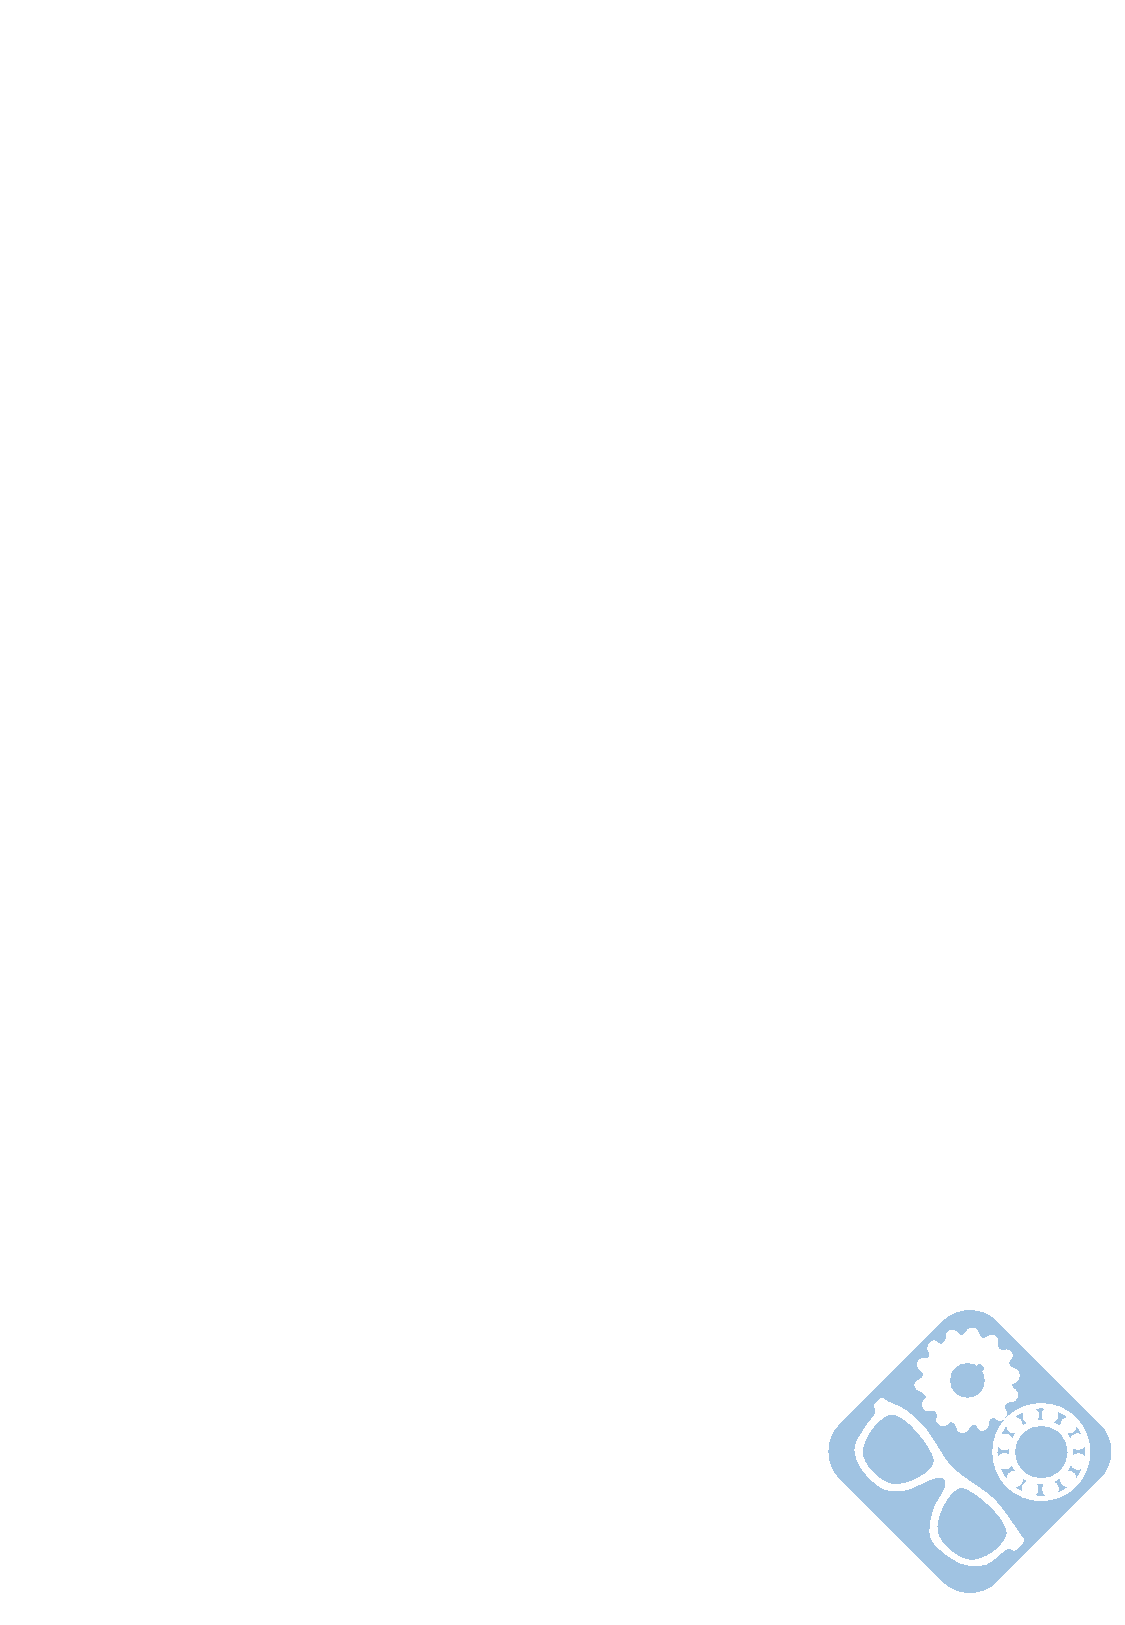
\includegraphics[width=\paperwidth,height=\paperheight,%
keepaspectratio]{../../../img/fond4}%
\end{center}
\vfill
}}}

\begin{document}

\pagestyle{empty}

\AddToShipoutPicture*{\BackgroundPic}


\includegraphics[width=2cm]{../../../img/logo}

\Huge{DS \numero - \sujet}

\vspace{1cm}

\ifdef{\prive}{\begin{center}\colorbox{danger}{\Huge{Avec Correction}}\end{center}}{}

\begin{center}
\centering\huge{PTSI}
\end{center}

\vspace{2cm}


\begin{center}
\centering\Large{\jour}
\end{center}

\vspace{2cm}

\normalsize

\tableofcontents

\newpage

\AddToShipoutPicture{\BackgroundPicdeux}

\pagestyle{fancy}

\begin{center}
\Huge \sujet
\end{center}


\normalsize


\section{Contexte}

Les recours aux opérations chirurgicales pour traiter les pathologies cardiaques sont de plus en plus courants. La plupart de ces opérations est actuellement réalisée après avoir arrêté le c\oe ur du patient et mis en place une circulation et une oxygénation extérieures du sang. Cette procédure et les suites opératoires sont lourdes.
Il est possible d'opérer sans arrêter le c\oe ur, mais ce type d'opération à c\oe ur battant est plus délicat pour le chirurgien à cause des mouvements de la zone à opérer dûs à la respiration et aux battements du c\oe ur. Les battements cardiaques, contrairement aux mouvements respiratoires, ne sont pas cycliques et engendrent un déplacement rapide de la zone à opérer. Une intervention robotisée type maître-esclave avec prise en compte des battements cardiaques pour le déplacement du robot esclave est compliquée et dangereuse.

Lors d'une opération à c\oe ur battant, un maintien mécanique de la zone à opérer est indispensable. Ce maintien en position est réalisé par un stabilisateur composé de deux doigts en contact avec la zone à opérer. Le déplacement de la zone à opérer est ainsi diminué. Le stabilisateur est lié à la table d'opération par une attache reconfigurable. La stabilisation (figure \ref{fig01}) peut être active ou passive. Dans le cas d'une stabilisation active, un actionneur génère une action mécanique de compensation dans le but de diminuer le mouvement de la zone à opérer qui n'a pas été filtré par le stabilisateur passif. Ce mouvement constitue un déplacement résiduel.

\begin{figure}[ht]
\begin{center}
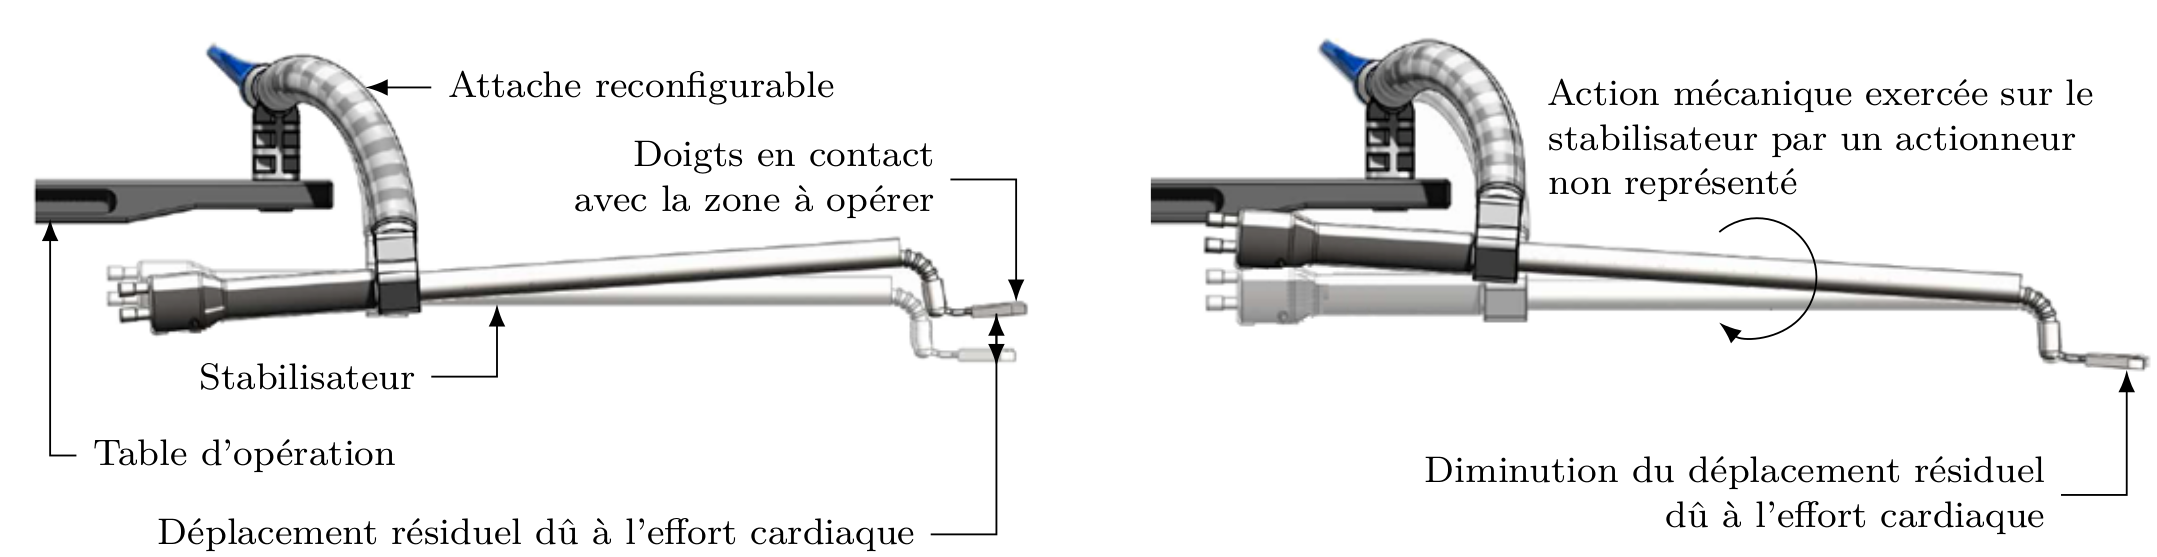
\includegraphics[width=0.9\linewidth]{img/fig01}
\caption{Stabilisations passive (à gauche) et active (à droite)}
\label{fig01}
\end{center}
\end{figure} 

\begin{figure}[ht]
\begin{center}
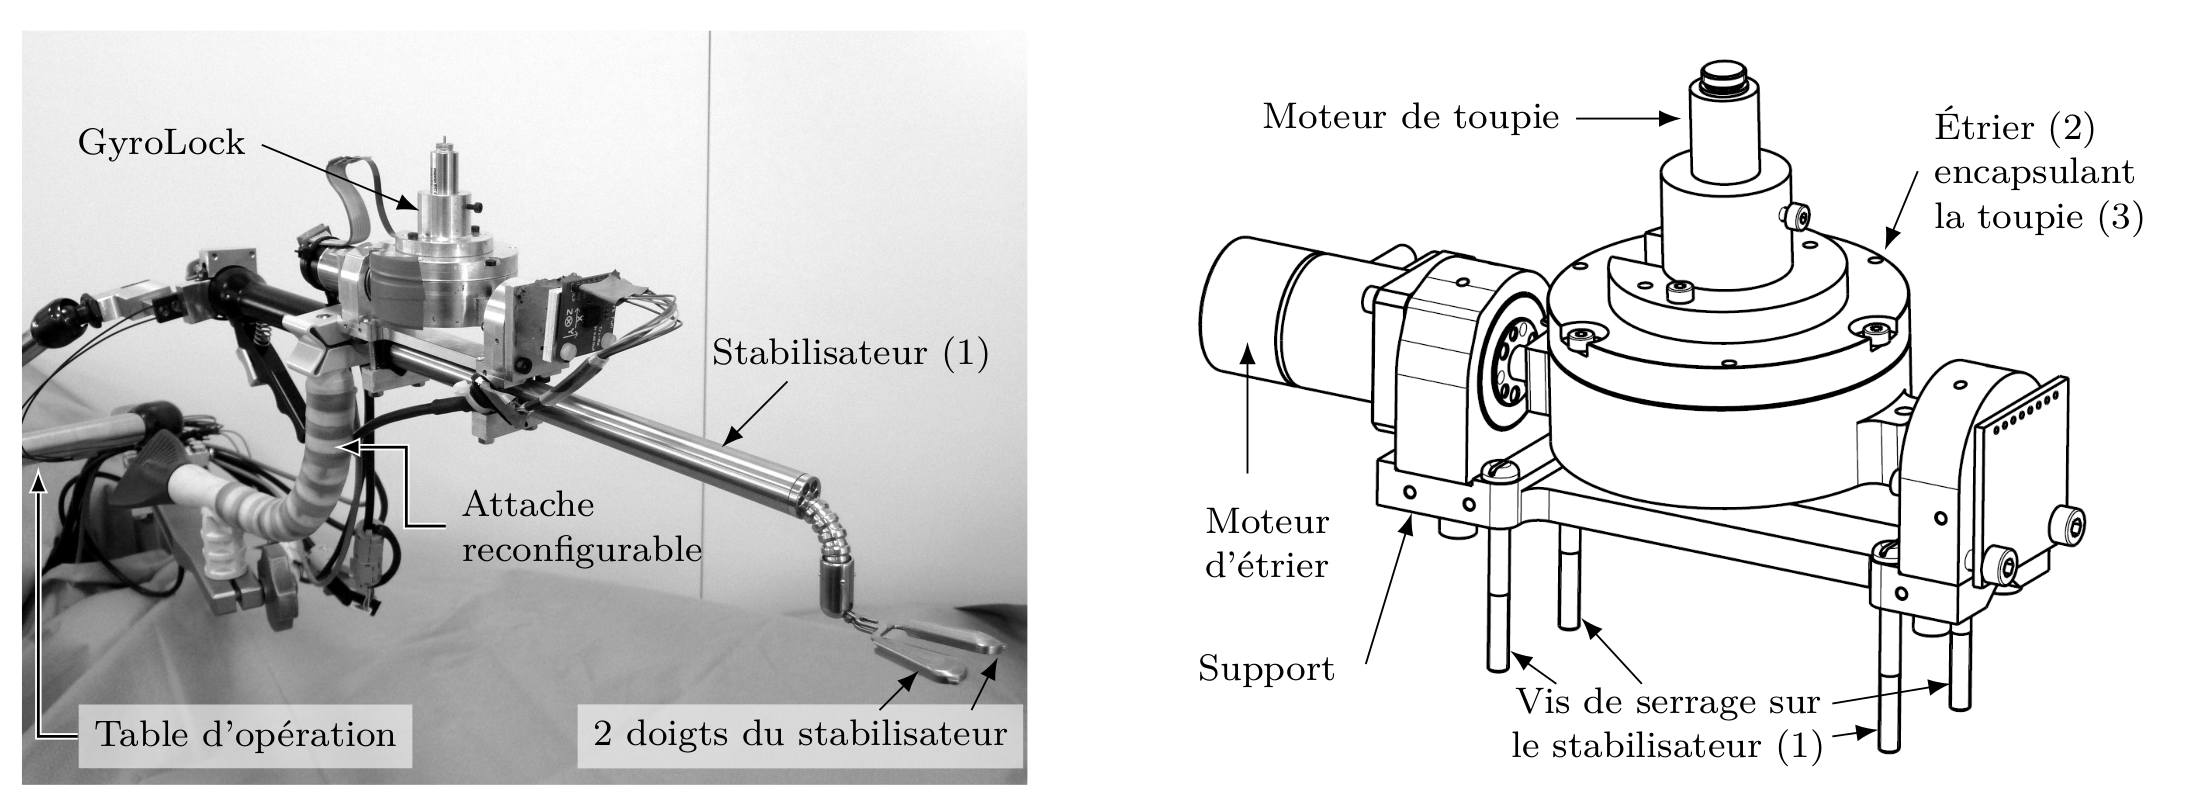
\includegraphics[width=0.8\linewidth]{img/fig02}
\caption{Photo du GyroLock installé sur un stabilisateur (à gauche) et son modèle volumique (à droite) }
\label{fig02}
\end{center}
\end{figure} 

\newpage

Ce système, nommé GyroLock, présente deux avantages par rapport aux autres stabilisateurs actifs existants : 
\begin{itemize}
 \item il peut être mis en place sur la plupart des stabilisateurs passifs afin de limiter l'investissement financier des structures hospitalières voulant s'équiper de stabilisateurs actifs ; 
 \item il ne nécessite pas de liaison avec la table d'opération donc le stabilisateur peut être placé dans n'importe quelle position. En effet, contrairement aux autres stabilisateurs actifs existants, le GyroLock ne comporte pas d'actionneur dont le stator est lié à la table d'opération.
\end{itemize}
 
Le GyroLock est muni de deux actionneurs. Le moteur de toupie met en rotation la toupie (3) par rapport à l'étrier (2) autour d'un axe initialement vertical. Un second moteur électrique, appelé moteur d'étrier, entraîne en rotation l'étrier (2) par rapport au support lié au stabilisateur (1) autour d'un axe colinéaire à la direction du stabilisateur (1). Cette seconde rotation génère un effet dynamique appelé effet gyroscopique. Cet effet peut être considéré comme une action mécanique permettant d'atténuer le déplacement résiduel de la zone à opérer en contact avec les doigts du stabilisateur (1). 

\paragraph{Exigences fonctionnelles} ~\ \\

Le diagramme des exigences partiel de la stabilisation cardiaque est donné figure \ref{fig03}.
 
\begin{figure}[ht]
\begin{center}
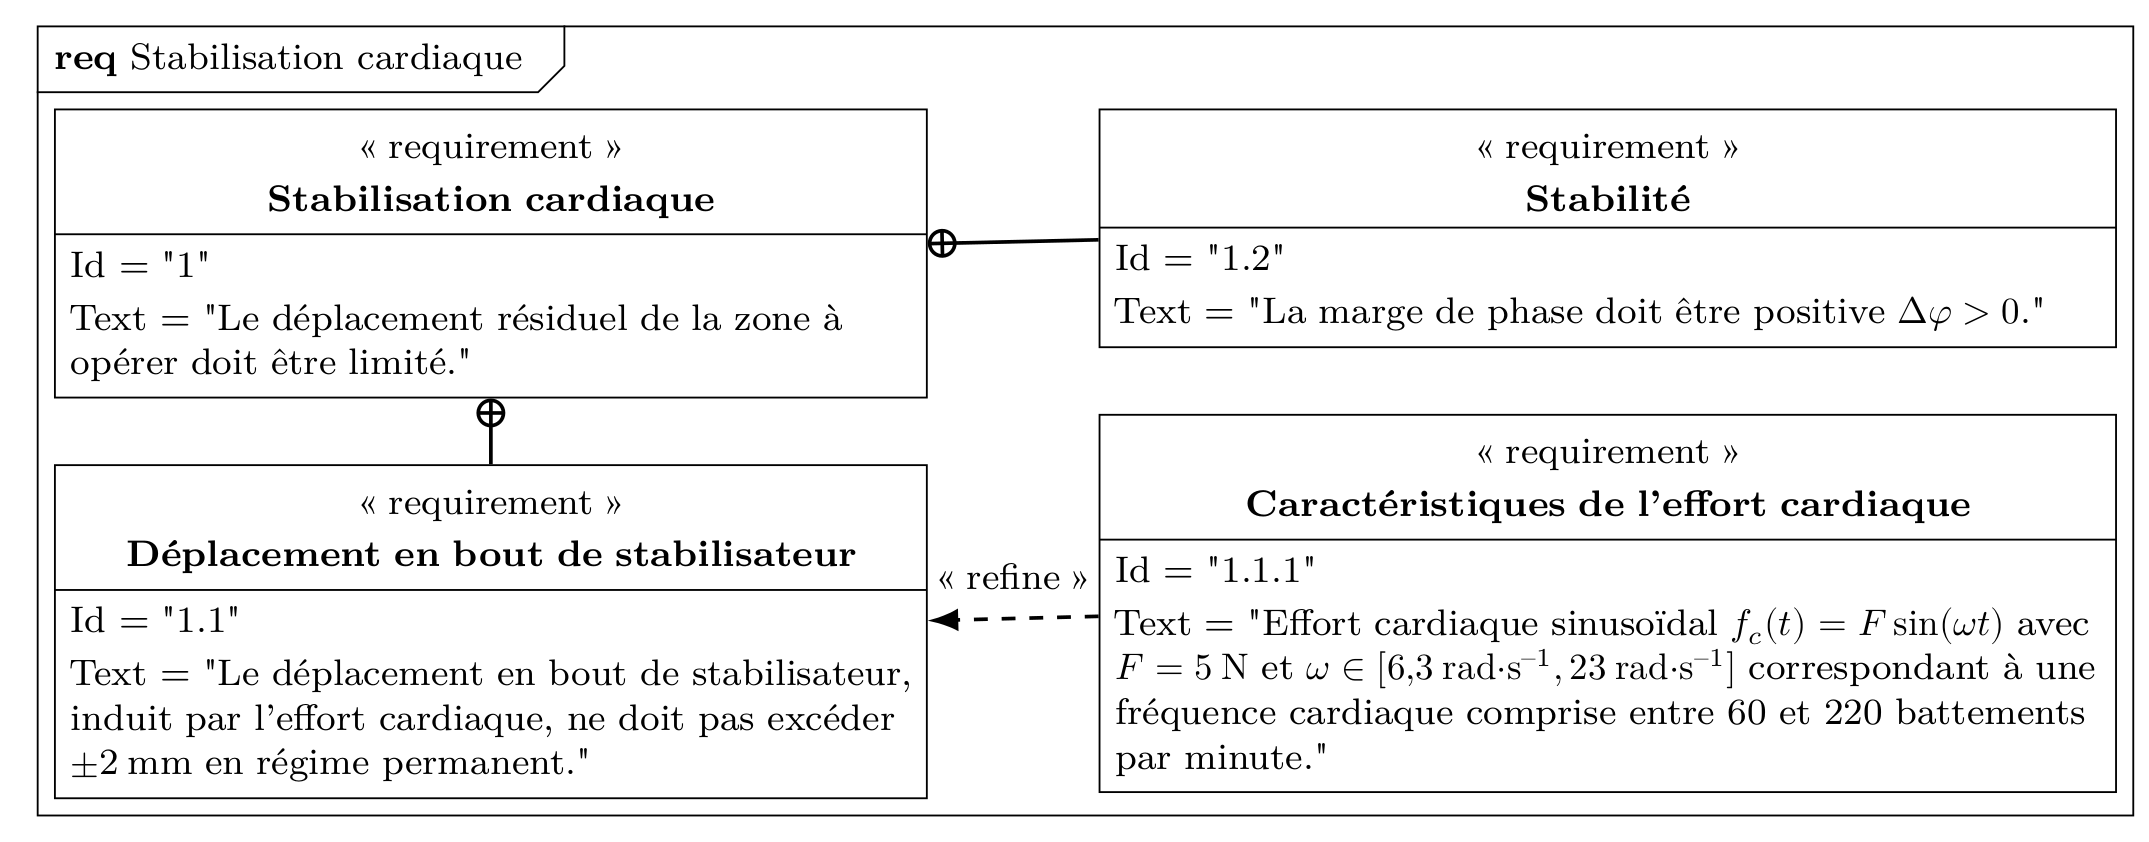
\includegraphics[width=0.95\linewidth]{img/fig03}
\caption{Diagramme des exigences partiel}
\label{fig03}
\end{center}
\end{figure} 

L'objectif de ce sujet est de montrer que l'utilisation d'un actionneur à effet gyroscopique permet d'améliorer le maintien de la zone à opérer. Les étapes nécessaires à la validation de cet objectif sont les suivantes : 
\begin{itemize}
 \item dans un premier temps, l'analyse de résultats expérimentaux permettra de modéliser le mécanisme ; 
 \item après avoir analysé l'effet gyroscopique et réglé le correcteur empêchant la dérive de l'étrier, une étude dynamique du stabilisateur permettra de déterminer un modèle de comportement du stabilisateur ; 
 \item enfin, la partie III traitera du choix d'une loi de commande permettant de respecter les exigences figure \ref{fig03}. 
\end{itemize}

\newpage

\section{Résultats expérimentaux et modélisation du mécanisme\label{partI}}

\paragraph{Objectif :} Exploiter les résultats d'une campagne expérimentale afin de modéliser la liaison entre la table d'opé­ration et le stabilisateur, puis exprimer le déplacement en bout de stabilisateur.

\subsection{Mesure du déplacement en bout de stabilisateur}

Un stabilisateur passif (sans système de stabilisation active) a été testé sur un sujet porcin de 40 kg sous assis­tance respiratoire et anesthésie générale. Les volume et fréquence respiratoires sont respectivement de 300 mL et 15,6 respirations par minute. Une mesure du déplacement et de l'effort cardiaque au bout du stabilisateur passif a été effectuée. 

Le système cardiovasculaire porcin étant similaire à celui d'un être humain, il est possible, grâce à une méthode non détaillée dans cette étude, d'estimer les valeurs équivalentes pour un homme de 90 kg. La figure \ref{fig04} donne l'évolution temporelle, pour un patient humain, du déplacement du point P situé au bout du stabilisateur (figure \ref{fig05}).

\begin{figure}[ht]
\begin{center}
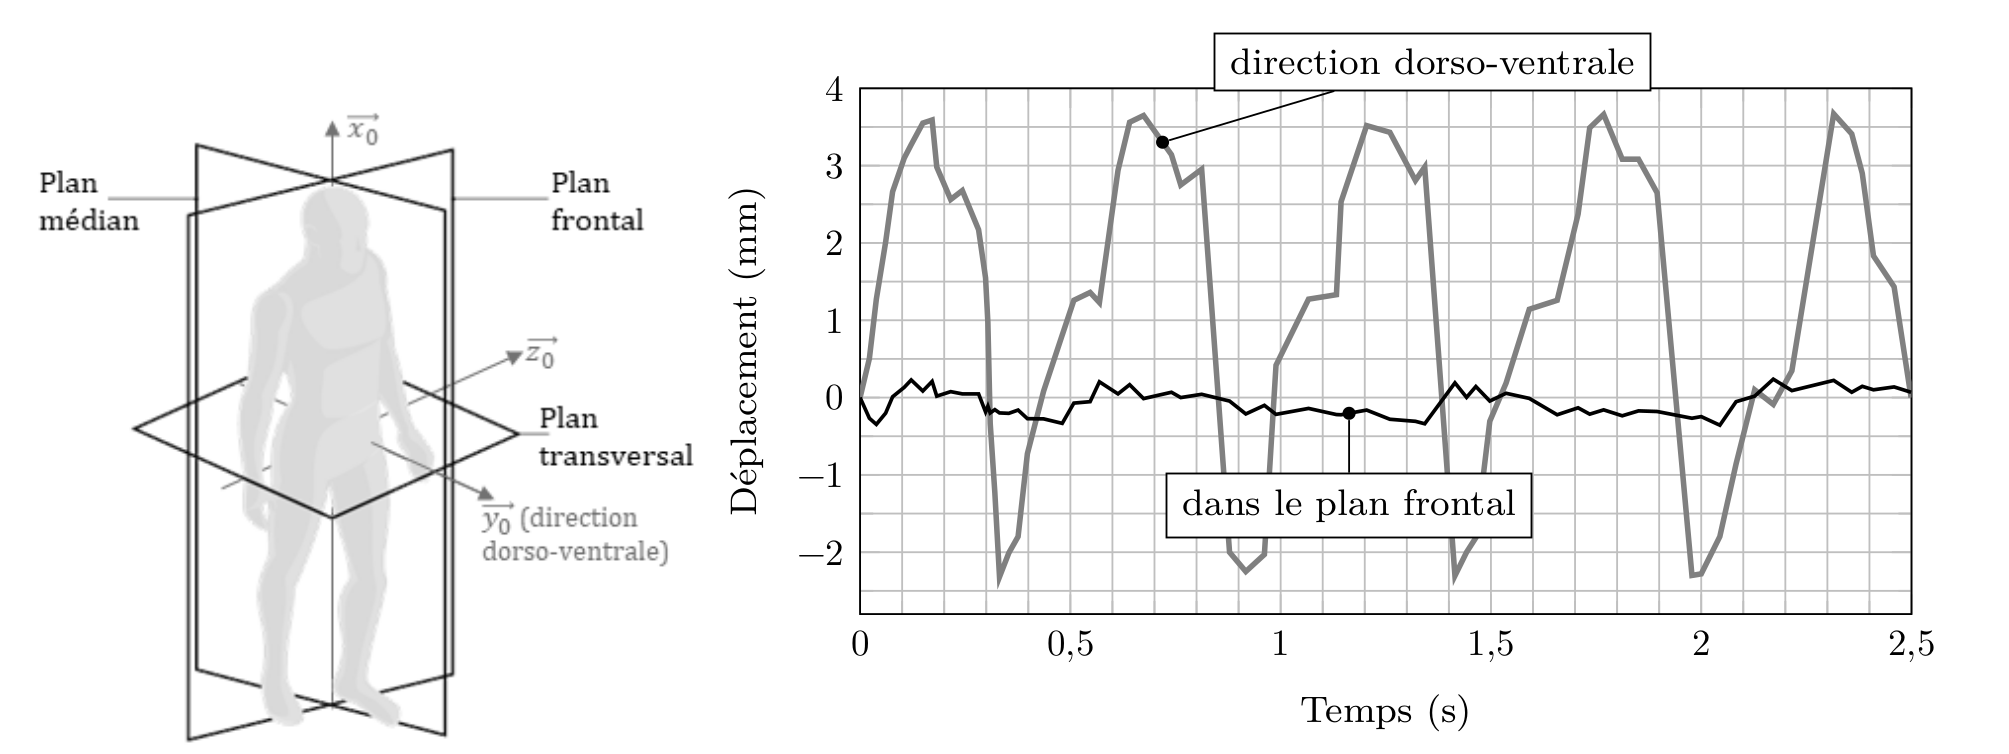
\includegraphics[width=0.9\linewidth]{img/fig04}
\caption{Plans anatomiques, déplacements résiduels dans le plan frontal et dans la direction dorso-ventrale}
\label{fig04}
\end{center}
\end{figure} 

\question{Déterminer, à partir de la figure \ref{fig04}, les valeurs minimales et maximales de déplacement du point P dans la direction dorso-ventrale, notées $u_{d}^{max}$ et $u_{d}^{min}$, et dans le plan frontal, notées $u_{f}^{max}$ et $u_{f}^{min}$ . Déterminer laquelle des deux stabilisations (passive ou active) est nécessaire pour respecter le diagramme des exigences figure \ref{fig03}.}

~\

La liaison entre le stabilisateur (1) et la table d'opération (0) sera modélisée de trois façons différentes selon la finalité :
\begin{itemize}
 \item par une liaison sphérique (partie \ref{partII2}) afin de déterminer quelles rotations doivent être prises en compte pour représenter le mouvement du stabilisateur par rapport à la table d'opération, 
 \item par un encastrement (partie \ref{partIII1}) afin d'étudier l'effet gyroscopique sans prendre en compte le mouvement du stabilisateur,
 \item par une liaison non parfaite (partie \ref{partIII3}) modélisant la flexibilité de l'attache reconfigurable. 
\end{itemize}

\subsection{Formulation du modèle de la liaison entre la table d'opération et le stabilisateur\label{partII2}}

La modélisation retenue pour estimer le déplacement du point P situé au bout du stabilisateur (1) est donnée figure \ref{fig05}. La direction $\overrightarrow{y_0}$ correspond à la direction dorso-ventrale, le plan $(O,\overrightarrow{x_0},\overrightarrow{y_0})$ est le plan frontal et l'axe « pied-tête » du patient est représenté par le vecteur $\overrightarrow{x_0}$. Le point $O_0$ est un point de référence choisi, considéré comme fixe par rapport à la table d'opération (0). 

\begin{figure}[ht]
\begin{center}
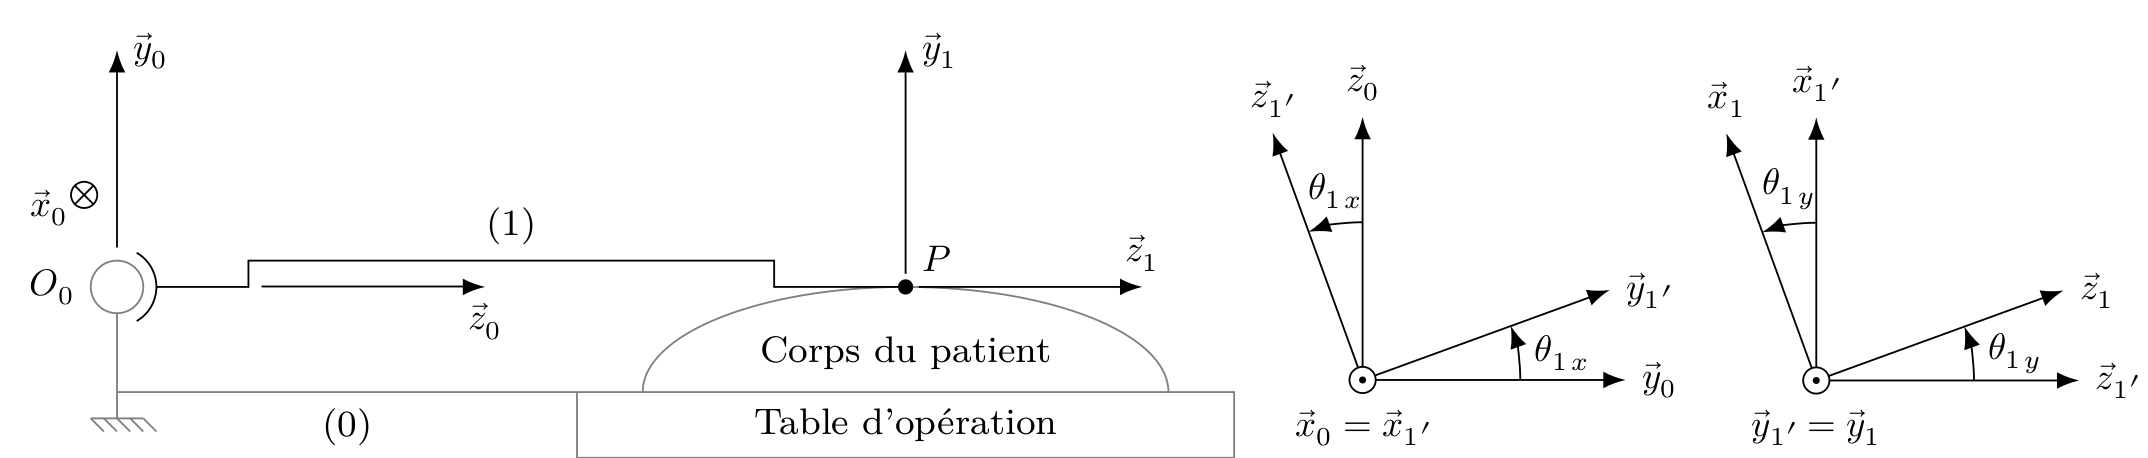
\includegraphics[width=0.95\linewidth]{img/fig05}
\caption{Modélisation du stabilisateur (1) en position de référence $(\theta_{1x}=\theta_{1y}=0)$ et figures de changement de base }
\label{fig05}
\end{center}
\end{figure}

Le déplacement du point P situé au bout du stabilisateur (1) correspond à une trop grande flexibilité de l'attache reconfigurable (figures \ref{fig01} et \ref{fig02}) utilisée pour lier le stabilisateur à la table d'opération (0). La liaison entre les solides (0) et (1) est modélisée par une liaison sphérique de centre $O_0$.

~\

Deux rotations successives permettent de positionner la base $B_1 (\overrightarrow{x_1},\overrightarrow{y_1},\overrightarrow{z_1})$ liée au stabilisateur par rapport à la base $B_0(\overrightarrow{x_0},\overrightarrow{y_0},\overrightarrow{z_0})$ liée à la table d'opération :
\begin{itemize}
 \item une rotation autour de $\overrightarrow{x_0}$ d'angle $\theta_{1x}$ permet de définir une base intermédiaire $B_1^{'}(\overrightarrow{x_0},\overrightarrow{y_{1'}},\overrightarrow{z_{1'}})$,
 \item une rotation autour de $\overrightarrow{y_{1'}}$  d'angle $\theta_{1y}$ permet d'orienter la base $B_1$ par rapport à la base $B_1^{'}$. 
\end{itemize}

~\

Les figures de changement de base sont données figure \ref{fig05}. La position du point P par rapport à la table d'opération (0) est donnée par $\overrightarrow{OP}=L\overrightarrow{z_1}$ avec $L=0,3m$. Le point $P_0$ tel que $\overrightarrow{O_0P_0}=L\overrightarrow{z_0}$ correspond à la position de référence du point P pour laquelle $\theta_{1x}=\theta_{1y}=0$.

\question{Exprimer le vecteur $\overrightarrow{P_0P}$ dans la base $B_0$. En déduire l'expression de $u_d=\overrightarrow{P_0P}\cdot \overrightarrow{y_0}$ correspondant au déplacement en bout de stabilisateur dans la direction dorso-ventrale et $u_f= \ \parallel \overrightarrow{P_0P}-u_d\cdot \overrightarrow{y_0} \ \parallel$ traduisant le déplacement en bout de stabilisateur dans le plan frontal.}

\question{Déterminer les expressions linéarisées à l'ordre 1 de $u_d$ et $u_f$ ($\theta_{1x}$ et $\theta_{1y}$ sont proches de 0). En utilisant le résultat de la question 1, donner la valeur numérique (en radian) des débattements angulaires $\Delta\theta_{1x}=max(\theta_{1x})-min(\theta_{1x})$ et $\Delta\theta_{1y}$ du stabilisateur. En déduire qu'une rotation peut être négligée (en précisant laquelle et en justifiant). En supposant la rotation d'axe $(O_0,\overrightarrow{z_0})$ est également négligeable, proposer une \og nouvelle \fg liaison (en précisant ses caractéristiques géométriques) modélisant le mouvement du stabilisateur (1) par rapport à la table d'opération (0).}

\question{Préciser alors la direction du moment de compensation que devra générer le système Gyrolock afin de réduire le déplacement du point P.}

\newpage

\section{Effet gyroscopique et modélisation du stabilisateur}

\paragraph{Objectif :} Étudier les actions mécaniques créées par le système GyroLock, définir et régler la chaine d'asservis­sement de l'étrier puis modéliser le comportement du stabilisateur grâce à une étude dynamique. 

\subsection{Étude de l'effet gyroscopique généré par le système GyroLock\label{partIII1}}

Pour déterminer les actions mécaniques créées par le système GyroLock sur le stabilisateur (1), un modèle simplifié du mécanisme, donné figure \ref{fig06}, est utilisé.

Ce modèle simplifié, dans lequel la liaison entre le stabilisateur (1) et la table d'opération (0) est modélisée par un encastrement, permet : 
\begin{itemize}
 \item d'étudier l'effet gyroscopique $c_x(t)$ créé par le système GyroLock permettant de compenser l'effet de l'effort cardiaque, sans prendre en compte le mouvement du stabilisateur (1) ; 
 \item de déterminer les conditions d'utilisation du système GyroLock afin de minimiser les autres actions méca­niques créées et considérées comme indésirables. 
\end{itemize}

\begin{figure}[ht]
\begin{center}
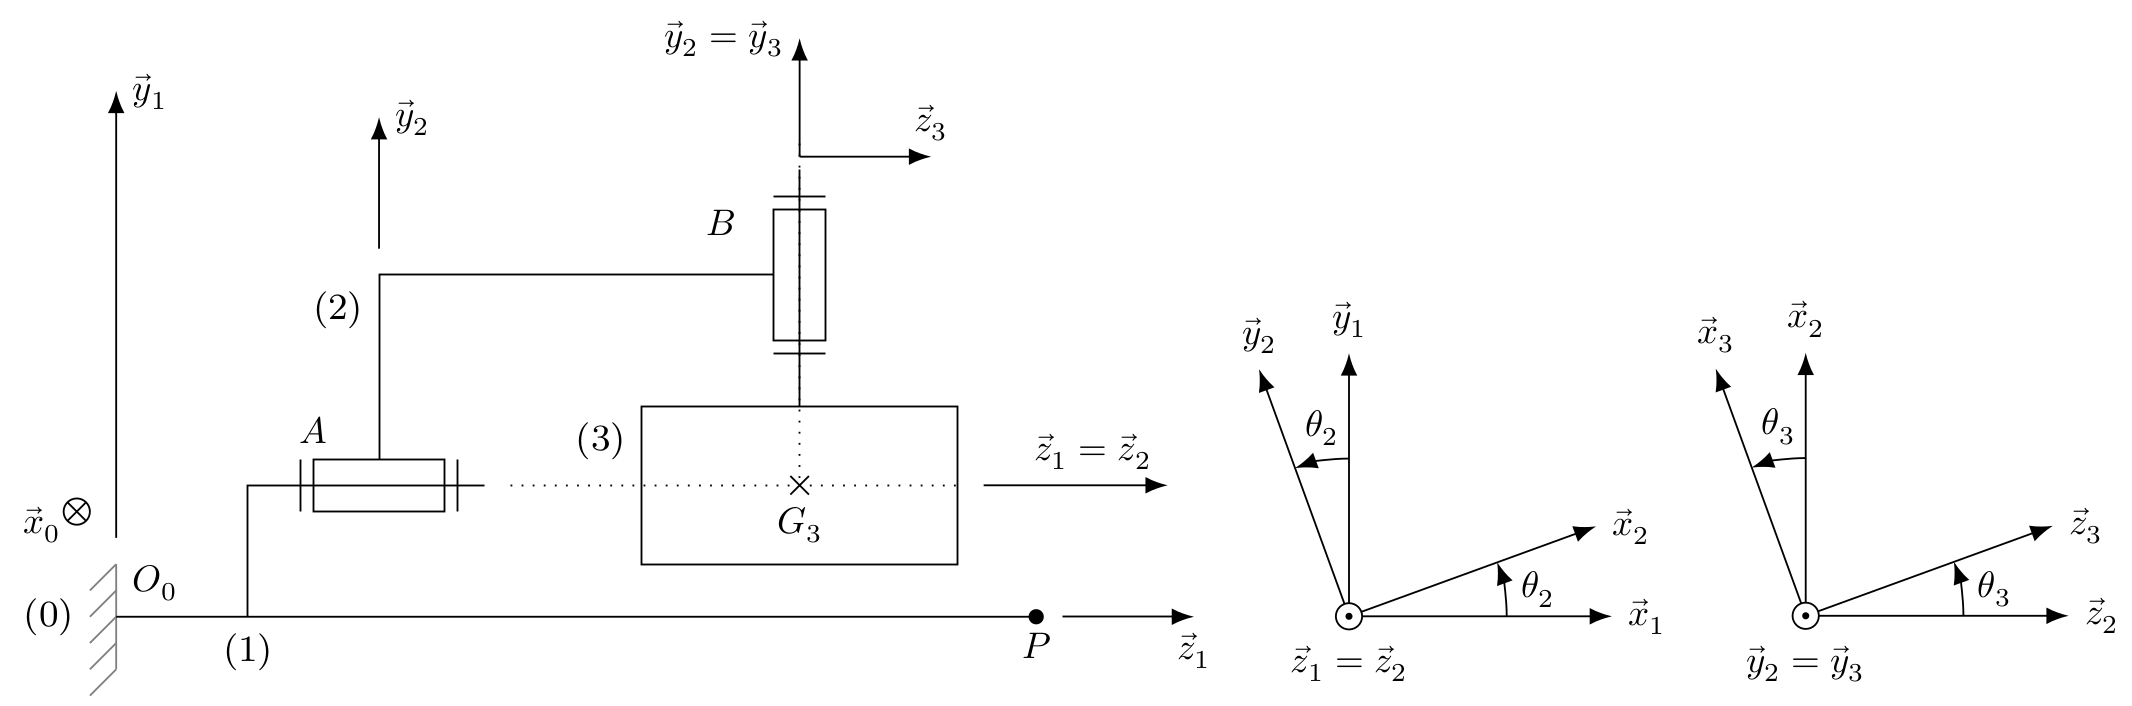
\includegraphics[width=0.8\linewidth]{img/fig06}
\caption{Schéma cinématique simplifié du mécanisme (représenté pour $\theta_2=\theta_3=0$) et figures de changement de base }
\label{fig06}
\end{center}
\end{figure}

Le système GyroLock, dont la modélisation est donnée figure \ref{fig06}, est composé de trois solides :
\begin{itemize}
 \item le support, relié au stabilisateur (1) de repère associé $R_1(0_0,\overrightarrow{x_1},\overrightarrow{y_1},\overrightarrow{z_1})$, en liaison encastrement au point $O_0$ avec la table d'opération (0),
 \item l'étrier (2) de repère associé $R_2(A,\overrightarrow{x_2},\overrightarrow{y_2},\overrightarrow{z_2}=\overrightarrow{z_1})$ tel que $\theta_2=(\overrightarrow{x_1},\overrightarrow{x_2})=(\overrightarrow{y_1},\overrightarrow{y_2})$,
 \item la toupie (3) de repère associé $R_3(B,\overrightarrow{x_3},\overrightarrow{y_2}=\overrightarrow{y_3},\overrightarrow{z_3})$ tel que $\theta_3=(\overrightarrow{x_2},\overrightarrow{x_3})=(\overrightarrow{z_2},\overrightarrow{z_3})$.
\end{itemize}

~\

Les figures de changement de base sont données figure \ref{fig06}. Toutes les liaisons sont supposées parfaites et les caractéristiques inertielles des solides sont les suivantes:
\begin{itemize}
 \item étrier (2): masse et inertie négligeables,
 \item toupie (3): masse m3, centre d'inertie $G_3$ tel que $\overrightarrow{O_0G_3}=L_{G_3}\overrightarrow{z_1}+H_{G_3}\overrightarrow{y_1}$. L'axe $(G_3,\overrightarrow{y_2}=\overrightarrow{y_3})$ étant un axe de symétrie de révolution de la toupie (3), sa matrice d'inertie au point $G_3$ s'exprime dans la base $B_2$ sous la forme $I(G_3,3)=\left[\begin{array}{ccc} 
         A_3&0&0 \\ 0&B_3&0 \\ 0&0&A_3 
   \end{array}\right]$
\end{itemize}

\newpage

Pour la modélisation des actions mécaniques extérieures, les hypothèses suivantes sont adoptées:
\begin{itemize}
 \item les actions mécaniques dues à la pesanteur sont négligées devant les effets dynamiques,
 \item l'action mécanique transmise par la liaison encastrement entre les solides (0) et (1) est modélisée au point $G_3$ par
$\left \{T_{0 \rightarrow 1}\right \}=\left \{
\begin{matrix}
 X_{01}\overrightarrow{x_1}+Y_{01}\overrightarrow{y_1}+Z_{01}\overrightarrow{z_1} \\ 
 L_{01}\overrightarrow{x_1}+M_{01}\overrightarrow{y_1}+N_{01}\overrightarrow{z_1}
\end{matrix}
\right \}_{G_3}
$
\end{itemize}

Le référentiel $R_0(O_0,\overrightarrow{x_0},\overrightarrow{y_0},\overrightarrow{z_0})$ lié à la table d'opération (0) est galiléen.

\question{Compléter le graphe d'analyse mécanique fourni sur le document réponse.}

~\

On isole le système $\Sigma=\{1,2,3 \}$.

\question{En tenant compte des hypothèses faites, faire le bilan des actions mécaniques extérieures à $\Sigma=\{ 1,2,3 \}$.}

~\

On cherche à exprimer les composantes $L_{01}$,  $M_{01}$ et  $N_{01}$ en fonction de $\theta_2$, $\theta_3$, $\dot{\theta}_2$, $\dot{\theta}_3$, $A_3$ et $B_3$. Il faut alors appliquer le principe fondamental de la dynamique au système isolé $\Sigma$ dans le référentiel galiléen (pas encore abordé en PTSI), plus particulièrement l'équation de moment écrite en $G_3$ :
$\overrightarrow{\delta}(G_3,3/0)=\Sigma\overrightarrow{M}(G_3, ext\rightarrow\Sigma=\{ 1,2,3 \})$.

\question{Exprimer $\Sigma\overrightarrow{M}(G_3, ext\rightarrow\Sigma=\{ 1,2,3 \})$, la somme des moments s'appliquant sur $\Sigma$ en $G_3$.}

~\

En négligeant les inerties de (1) et (2), la définition du moment dynamique au point $G_3$ du solide (3) en mouvement dans le référentiel galiléen $R_0$ s'écrit: $\overrightarrow{\delta}(G_3,3/0)=\left [ \frac{ \mathrm{d} \overrightarrow{\sigma}(G_3,3/0)}{ \mathrm{d} t} \right]_{R_0}$ .

L'expression du moment cinétique au point $G_3$ du solide (3) en mouvement dans le référentiel galiléen $R_0$ est la suivante:
$\overrightarrow{\sigma}(G_3,3/0)=B_3 \dot{\theta_3}\overrightarrow{y_2}+A_3\dot{\theta_2}\overrightarrow{z_2}$.

\question{En déduire l'expression de $\overrightarrow{\delta}(G_3,3/0)$ dans la base $B_2$.}

~\

On rappelle que $\overrightarrow{\delta}(G_3,3/0)=\Sigma\overrightarrow{M}(G_3, ext\rightarrow\Sigma=\{ 1,2,3 \})$.

\question{Grâce aux expressions trouvées précédemment, et en les projetant dans $B_1$, écrire les 3 équations issues du principe fondamental de la dynamique appliqué à $\Sigma$ dans $R_1$.}

~\

Lorsque la toupie (3) tourne avec une  vitesse constante $\omega_3=\dot{\theta}_3$ par rapport à l'étrier (2), l'expression des moments $L_{01}$, $M_{01}$ et $N_{01}$ donne le système suivant:
$\begin{cases}
 L_{01}(t)=-c_x(t)cos\theta_2(t) \\ 
 M_{01}(t)=-c_x(t)sin\theta_2(t) \\ 
 N_{01}(t)=A_3\ddot\theta_2(t) \\ 
\end{cases}$
\\ où $c_x(t)=B_3\omega_3\dot\theta_2(t)=K_3 \cdot \dot\theta_2(t)$ correspond à l'effet gyroscopique.

L'action du c\oe ur sur le stabilisateur est modélisée par un glisseur de résultante $\overrightarrow{R}_{c\rightarrow1}=f_c\overrightarrow{y_1}$ au point P tel que $\overrightarrow{O_0P}=L\overrightarrow{z_1}$.

Les moments $L_{01}$, $M_{01}$ et $N_{01}$ doivent rester faibles afin de limiter les déformations de l'attache reconfigurable liant le stabilisateur (1) à la table d'opération (0).

\question{En supposant que la toupie (3) tourne à vitesse constante par rapport à l'étrier (2), exprimer $\dot\theta_2$ en fonction de $K_3$, $\theta_2$, $f_c$ et $L-L_{G_3}$ permettant de garantir que $L_{01}=0$ et de compenser l'effet de l'effort cardiaque $f_c$ (Méthode : calculer $\Sigma\overrightarrow{M}(G_3, ext\rightarrow\Sigma=\{1,2,3\})$ en rajoutant $\overrightarrow{M}(G_3, c\rightarrow 1)$).}

\question{Donner une condition sur l'angle $\theta_2$ et sur l'accélération angulaire $\ddot\theta_2$ afin que les moments $M_{01}$ et $N_{01}$ soient faibles.}

~\

L'étrier (2) doit être piloté en vitesse de rotation pour que l'effet gyroscopique $c_x(t)=K_3\dot\theta_2(t)$ compense l'effet de l'effort cardiaque. La campagne expérimentale présentée en partie \ref{partI} a permis de déterminer que la fréquence fondamentale de l'effort cardiaque $f_c(t)$ est de 1,5Hz.

La réponse de l'étrier (2) sera considérée comme suffisamment réactive si le temps de réponse à 5\% de la vitesse $\dot\theta_2(t)=\omega_2(t)$ pour une consigne $\dot\theta_{c2}(t)=\omega_{c2}(t)$ en échelon est d'un ordre inférieur à la demi-période du signal perturbateur $f_c(t)$.

\begin{figure}[ht]
\begin{center}
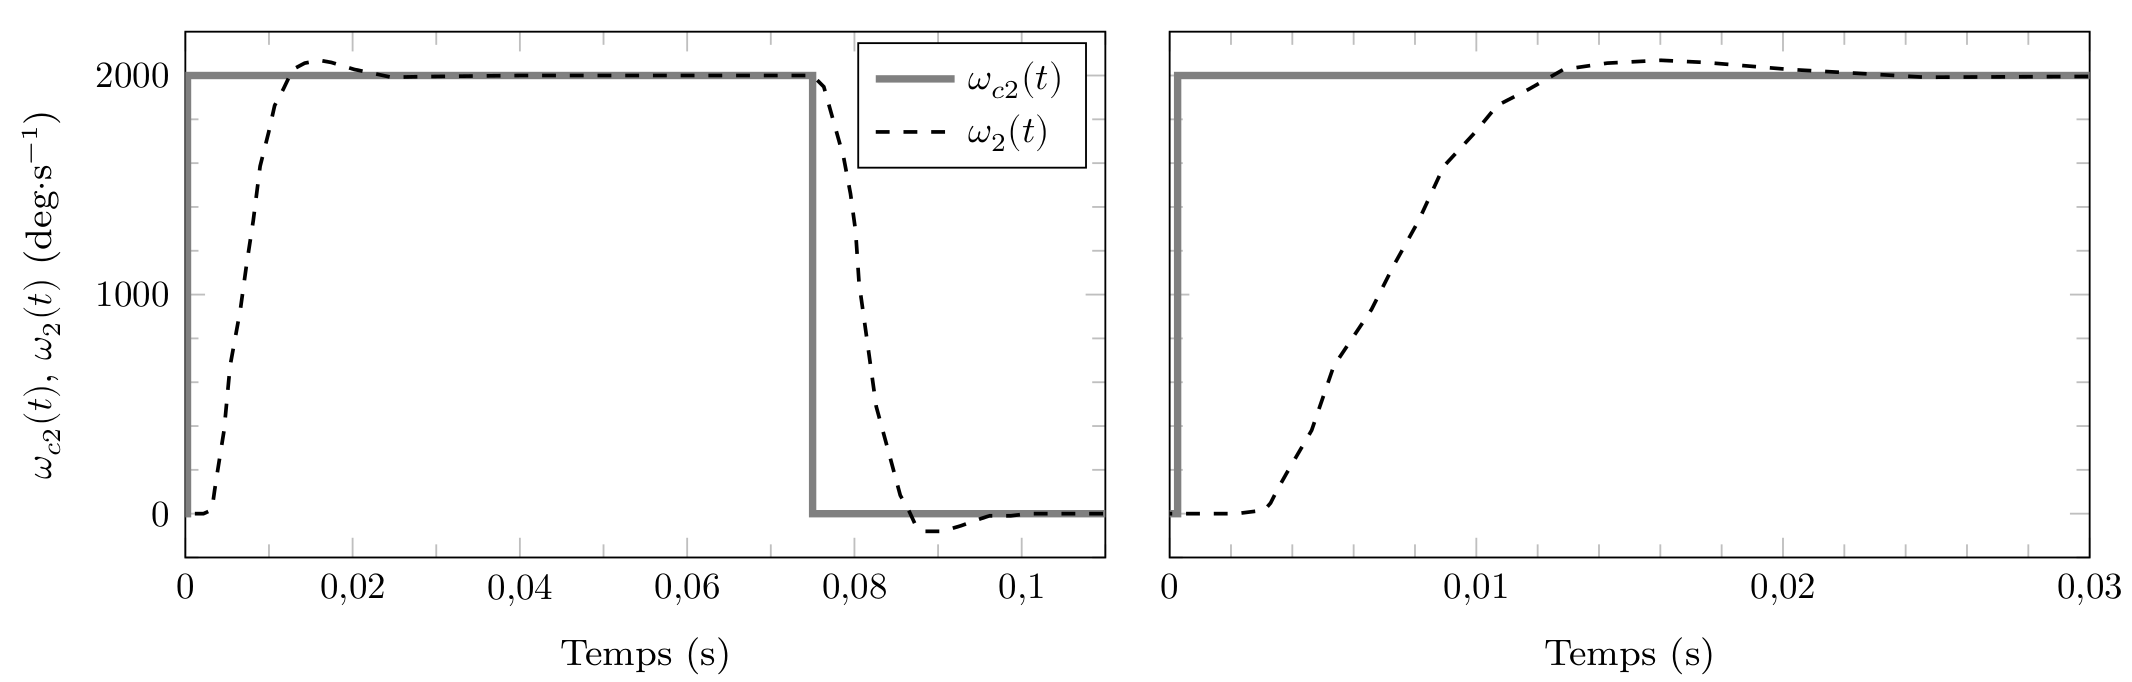
\includegraphics[width=0.8\linewidth]{img/fig07}
\caption{Réponse expérimentale de l'étrier et consigne associée (à droite, zoom sur le régime transitoire)}
\label{fig07}
\end{center}
\end{figure}

La réponse expérimentale à un échelon de vitesse $\Omega_{c2}(t)$ d'amplitude $2000\;deg\cdot s^{-1}$ est représentée figure \ref{fig07}.

Les transformées de Laplace de $\omega_2(t)$,  $\omega_{c2}(t)$,  $\theta_2(t)$ et $c_x(t)$ seront notées $\Omega_2(p)$, $\Omega_{c2}(p)$, $\Theta_2(p)$ et $C_x(p)$.

\question{Vérifier que la condition de réactivité énoncée ci-dessus est respectée. Justifier que la fonction de transfert de l'étrier (2) $H_2(p)=\frac{\Omega_2(p)}{\Omega_{c2}(p)}$ peut alors être approchée par un gain statique $K_2$ de valeur à préciser.}

~\

Il faut s'assurer que la position $\theta_2$ de l'étrier (2) ne s'éloigne pas trop de sa position de référence $\theta_2^*=0$. Le non-respect de cette condition, appelé dérive de l'étrier, génère un moment parasite $M_{01}$ responsable d'un déplacement du point P selon $\overrightarrow{x_1}$.

\subsection{Réglage du correcteur de la chaîne d'asservissement de l'étrier}

La figure \ref{fig08} montre la boucle d'asservissement sur la position $\theta_2$. $C(p)$ est la fonction de transfert d'un correcteur appelé correcteur d'étrier. La dérive de l'étrier sera évitée si $\lim\limits_{t \to \infty }\theta_2(t)=0$ lorsque la commande de l'étrier $U(p)$ est un échelon.

~\

Les 2 cas suivants sont envisagés:
\begin{itemize}
 \item avec une correction proportionnelle: $C(p)=K_{10}$,
 \item avec une correction proportionnelle-intégrale: $C(p)=K_{10}+\frac{K_{11}}{p}$.
\end{itemize}

\begin{figure}[ht]
\begin{center}
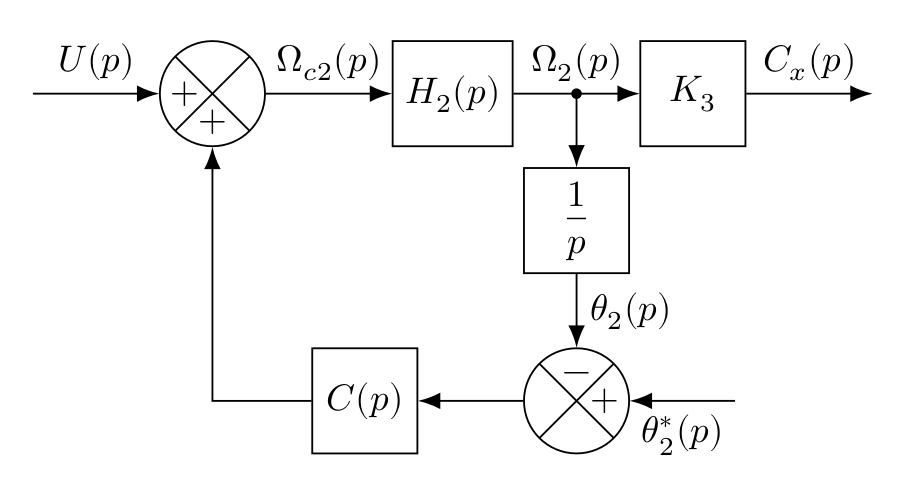
\includegraphics[width=0.5\linewidth]{img/fig08}
\caption{Asservissement de l'étrier}
\label{fig08}
\end{center}
\end{figure}

\question{Exprimer la fonction de transfert $H_{\theta_2}(p)=\frac{\theta_2(p)}{U(p)}$ avec $\theta_2^*(p)=0$ en fonction de $C(p)$ et $K_2$.}

\question{Déterminer $\lim\limits_{t \to \infty }\theta_2(t)$ lorsque $U(p)$ est un échelon unitaire pour la correction proportionnelle.}

\question{Déterminer $\lim\limits_{t \to \infty }\theta_2(t)$ lorsque $U(p)$ est un échelon unitaire pour la correction proportionnelle-intégrale.}

\question{Justifier la pertinence d'une correction proportionnelle-intégrale au regard de la problématique de la dérive de l'étrier.}

~\

Dans la suite de l'étude, le correcteur adopté est $C(p)=K_{10}+\frac{K_{11}}{p}$. 

L'effet gyroscopique $c_x(t)$ est lié à la vitesse de rotation $\omega_2(t)$ et la consigne $\theta_2^*(t)$ est maintenue à 0 pour éviter la dérive de l'étrier. La fonction de transfert utilisée pour modéliser le comportement de l'étrier (2) est notée $H_m(p)=\frac{\Omega_2(p)}{U(p)}$.

\question{Exprimer sous forme canonique la fonction de transfert $H_m(p)$ en fonction de $K_2$, $K_{10}$ et $K_{11}$.}

~\

Le calcul des gains $K_{10}$ et $K_{11}$ doit répondre aux deux exigences suivantes : permettre d'éviter la dérive de l'étrier (2) et ne pas ralentir le système, d'où le choix d'une fonction de transfert $H_m(p)$ caractérisée par un amortissement $\xi_m=0,37$ et une pulsation propre $\omega_m=2,45\;rad\cdot s^{-1}$.

\question{Déterminer les valeurs numériques de $K_{10}$ et $K_{11}$ au regard de ces exigences.}

~\

La rotation du stabilisateur (1) étudiée en partie \ref{partI} n'est pas prise en compte figure \ref{fig06}. Il est indispensable de considérer la flexibilité de l'attache reconfigurable utilisée pour lier le stabilisateur (1) à la table d'opération (0).

\subsection{Comportement dynamique du stabilisateur\label{partIII3}}

Dans la modélisation retenue (figure \ref{fig09}), une liaison pivot non parfaite permet de représenter la flexibilité de l'attache reconfigurable. La table d'opération (0) est supposée fixe et le référentiel $R_0(O_0,\overrightarrow{x_0},\overrightarrow{y_0},\overrightarrow{z_0})$ lié à la table (0) est galiléen. Au stabilisateur (1) est associé le repère $R_1(O_0,\overrightarrow{x_0}=\overrightarrow{x_1},\overrightarrow{y_1},\overrightarrow{z_1})$ avec $\theta_1=(\overrightarrow{y_0},\overrightarrow{y_1})=(\overrightarrow{z_0},\overrightarrow{z_1})$ . Le point $P$ tel que $O_0P=L$ représente le bout du stabilisateur (1) en contact avec la zone à opérer. 

\begin{figure}[ht]
\begin{center}
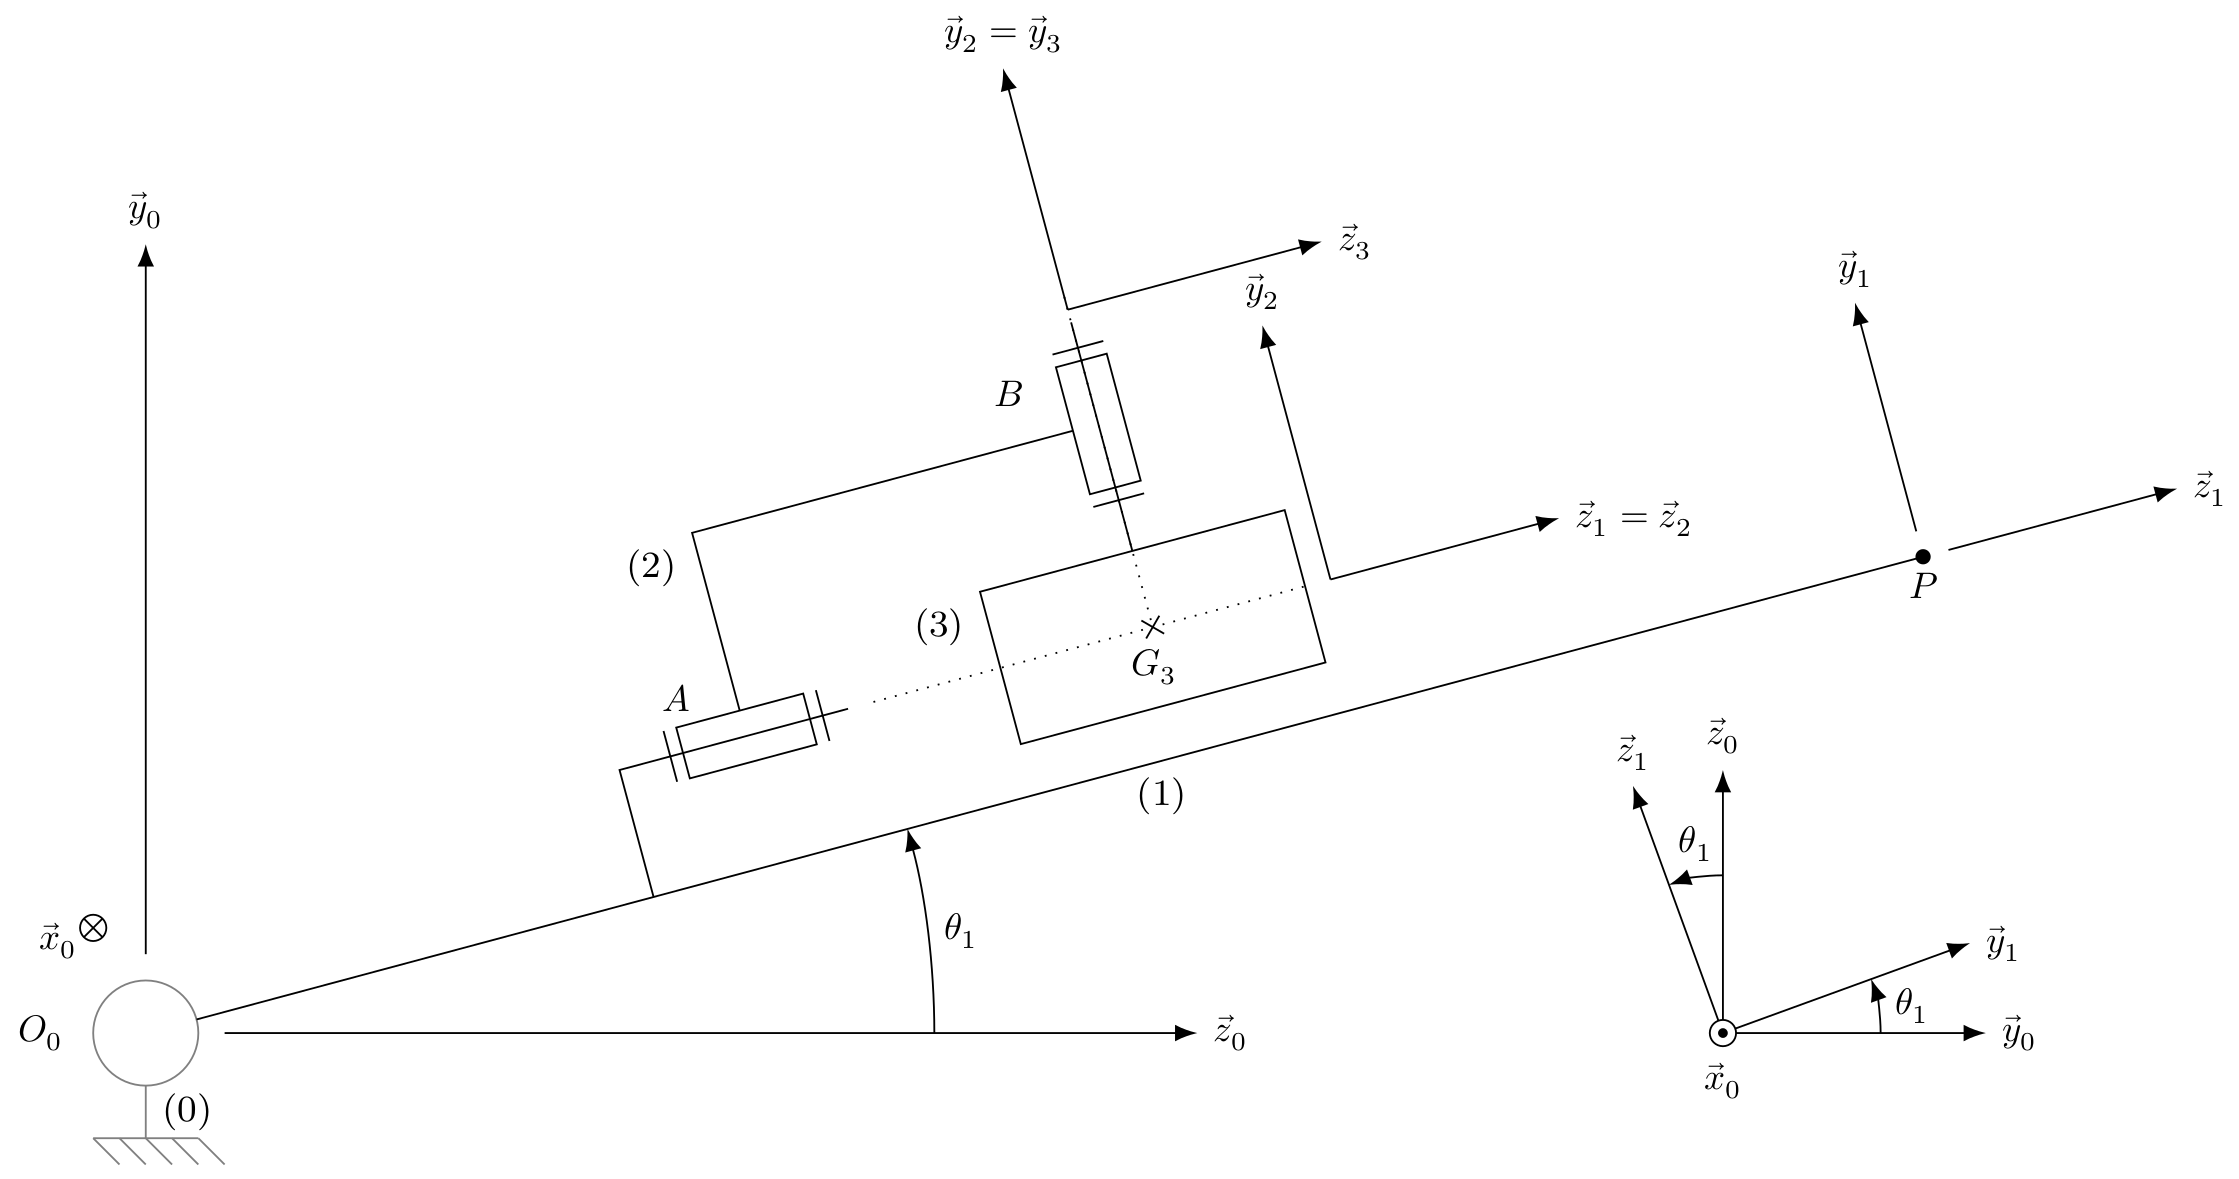
\includegraphics[width=0.8\linewidth]{img/fig09}
\caption{Modèle cinématique du système GyroLock (représenté pour $\theta_2=\theta_3=0$)}
\label{fig09}
\end{center}
\end{figure}


\paragraph{Paramétrage, notations et hypothèses}

\begin{itemize}
 \item la liaison pivot d'axe $(O_0,\overrightarrow{x_0})$ entre les solides (0) et (1) possède une raideur $k$ et un coefficient de frottement visqueux $f$, d'où $\overrightarrow{M}(O_0,\;0 \rightarrow 1)\cdot \overrightarrow{x_0}=-(k\theta_1+f\dot\theta_1)$,
 \item les autres liaisons sont supposées parfaites,
 \item l'action du coeur sur le stabilisateur (1) est modélisée par 
$\left \{T_{c \rightarrow 1}\right \}=\left \{
\begin{matrix}
 f_c \cdot \overrightarrow{y_1} \\ 
 \overrightarrow{0}
\end{matrix}
\right \}_{P}$,
 \item seul le déplacement vertical du point $P$ est pris en compte. On note $y(t)=-\overrightarrow{O_0P} \cdot \overrightarrow{y_0}$,
 \item le stabilisateur (1) est de masse $m_1$ et possède un centre d'invertie $G_1$ tel que $\overrightarrow{O_0G_1}=L_{G_1} \cdot \overrightarrow{z_1}$ et l'opérateur d'inertie est $I(G_1,1)=\left[\begin{array}{ccc} 
         A_1&0&0 \\ 0&A_1&0 \\ 0&0&C_1 
   \end{array}\right]_{B_1}$,
 \item la masse et l'inertie de l'étrier (2) sont négligeables,
 \item la toupie (3) est de masse $m_3$ et possède un centre d'invertie $G_3$ tel que $\overrightarrow{O_0G_3}=L_{G_3} \cdot \overrightarrow{z_1}+H_{G_3}\cdot \overrightarrow{y_1}$,
 \item les figures de changement de base sont données figures \ref{fig06} et \ref{fig09},
 \item les actions mécaniques dues à la pesanteur sont négligées devant les effets dynamiques,
 \item la loi de mouvement du stabilisateur (1) peut être mise sous la forme suivante : \\
$J_x\ddot\theta_1(t)+f\cdot \dot\theta_1(t)+k\cdot\theta_1(t)=c_x(t)-L\cdot f_c(t)$,\\ avec $J_x=A_1+A_3+m_1L^2_{G1}+m_3L^2_{G3}+m_3H^2_{G3}$.
\end{itemize}

~\

En supposant que $\theta_1$ reste proche de 0, la relation $y(t)=L\cdot \theta_1(t)$ sera utilisée.

Les transformées de Laplace de $y(t)$, $c_x(t)$ et $f_c(t)$ sont notées $Y(p)$, $C_x(p)$ et $F_c(p)$.

\question{Déterminer les expressions littérales des fonctions de transfert $H_{pert}(p)$ et $H_1(p)$ du schéma bloc figure \ref{fig10} en fonction de $L$, $J_x$, $f$ et $k$.}

\newpage

\begin{figure}[ht]
\begin{center}
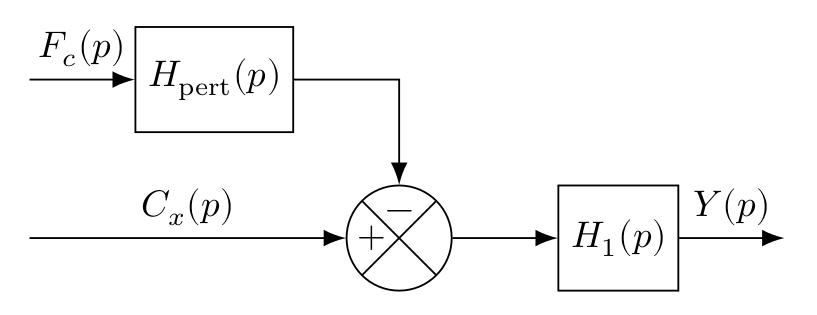
\includegraphics[width=0.5\linewidth]{img/fig10}
\caption{Schéma bloc du stabilisateur (1)}
\label{fig10}
\end{center}
\end{figure}

On rappelle que $L=0,3m$ et les valeurs retenues pour $J_x$, $f$ et $k$ sont :
\begin{itemize}
 \item $J_x=1,14\cdot 10^{-2}kg\cdot m^2$,
 \item $f=64\cdot 10^{-3}N\cdot m \cdot s \cdot rad^{-1}$,
 \item $k=95N\cdot m \cdot rad^{-1}$.
\end{itemize}

\question{Écrire $H_1(p)$ sous forme canonique, puis donner les expressions littérales et numériques de ses paramètres caractéristiques: gain statique $K_1$, amortissement $\xi_1$ et pulsation propre $\omega_1$.}

\question{Indiquer sur le diagramme de Bode du document réponse les pentes en dB/decade sur la courbe en gain, indiquer la pulsation de résonance et donner la définition littérale de $\frac{\left| H(j\omega)_{max} \right|}{\left| H(0) \right|}$.}


\section{Réglage de la loi de commande du stabilisateur}

\paragraph{Objectif :} Régler une loi de commande permettant de respecter les exigences figure \ref{fig03}. 

Une solution pour améliorer la commande du système de stabilisation est testée (non étudiée ici, seuls les résultats sont à analyser vis-à-vis du cahier des charges).

L'exploitation des modèles conduit à une simulation numérique aux évolutions temporelles de $y(t)$ et de $\theta_2(t)$

\begin{figure}[ht]
\begin{center}
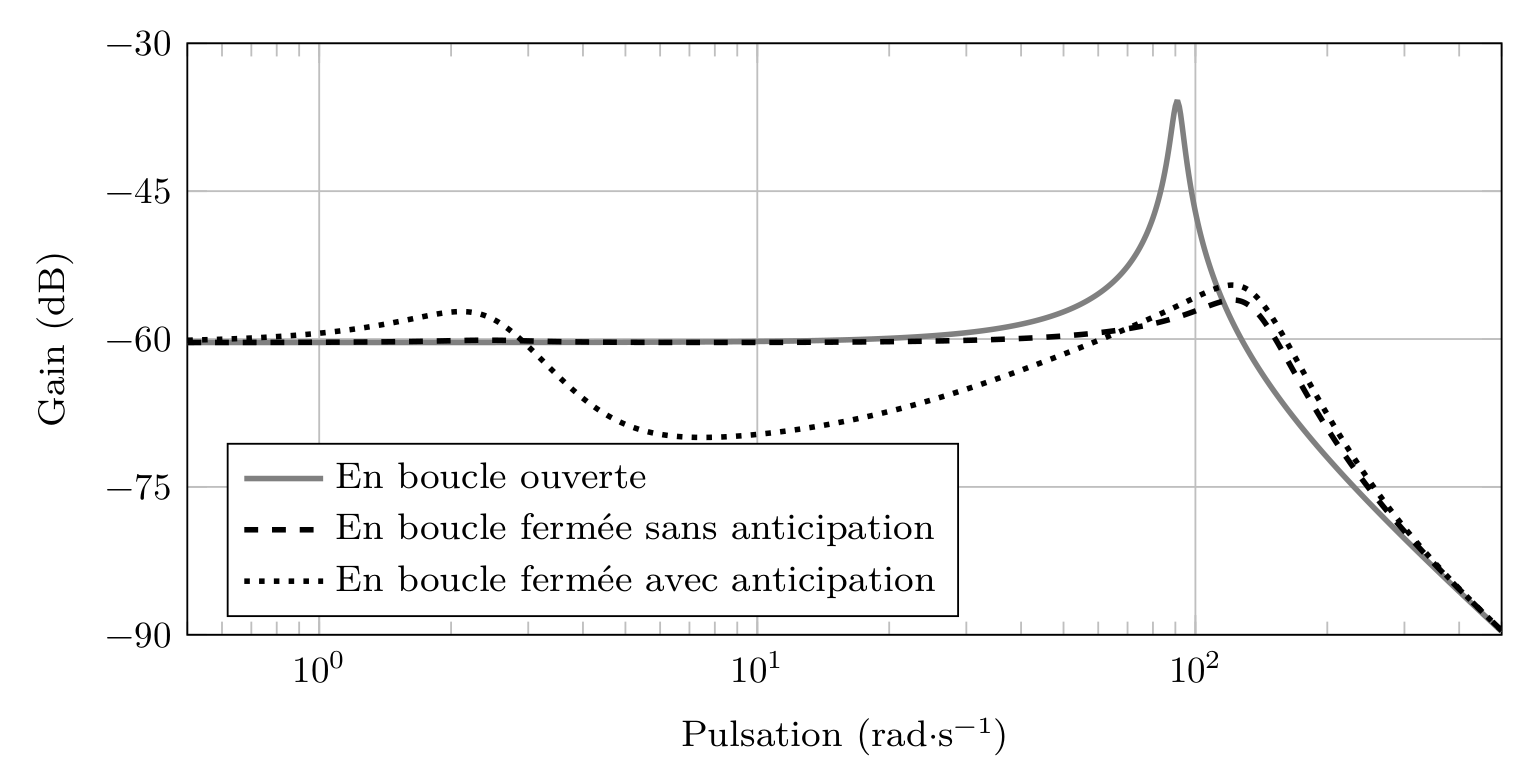
\includegraphics[width=0.8\linewidth]{img/fig17}
\caption{Réponses fréquentielles $|Y(j\omega)/F_c(j\omega)|$}
\label{fig17}
\end{center}
\end{figure}

\begin{figure}[ht]
\begin{center}
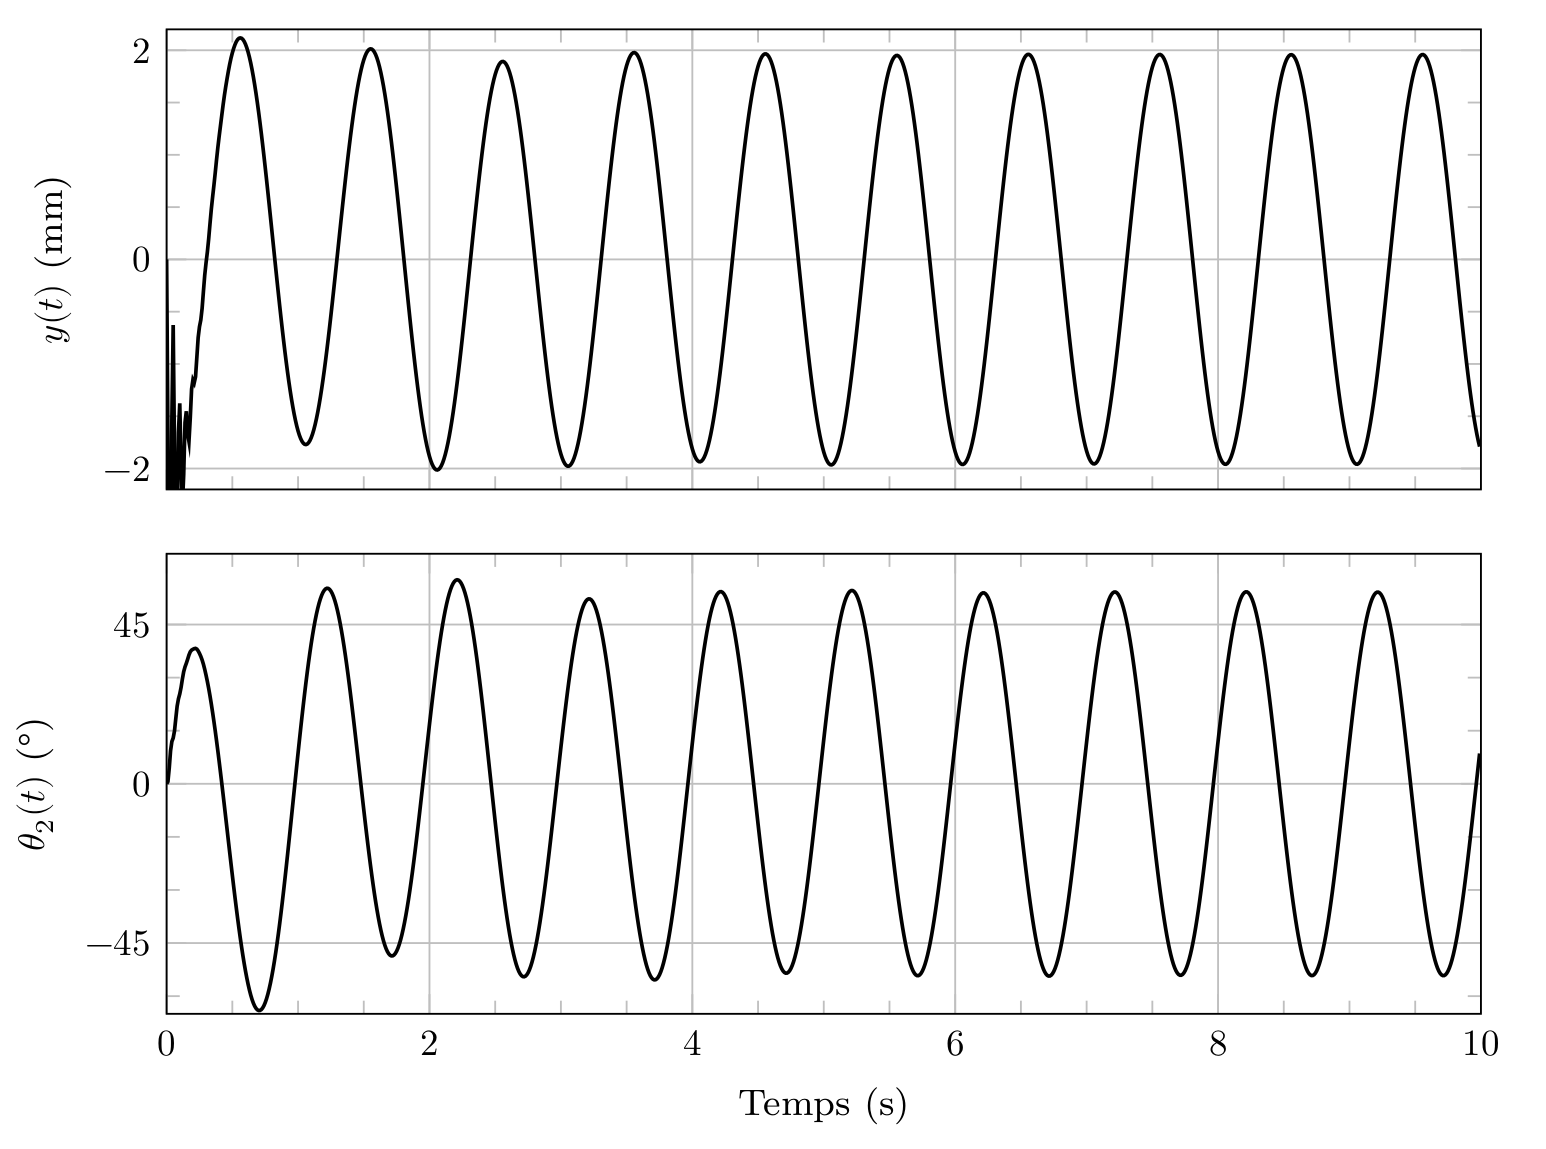
\includegraphics[width=0.68\linewidth]{img/fig18}
\caption{Évolutions temporelles de $v(t)$ et $\theta_2(t)$ avec estimation et compensation de $f_c(t)$.}
\label{fig18}
\end{center}
\end{figure}

\question{Analyser les courbes des figures \ref{fig17} et \ref{fig18} et les commenter vis-à-vis de l'exigence Id='1.1.1' (cf. diagramme des exigences fourni sur la figure \ref{fig03}). Conclure sur la capacité du GyroLock, tel qu'il a été modélisé dans cette étude, à maintenir la zone à opérer lors d'une opération à copieur battant.}

\section{Choix matériau-procédé}

\paragraph{Objectif :} Choisir un matériau compatible avec les contraintes subies par une pièce du stabilisateur (toupie).

\begin{figure}[ht]
\begin{center}
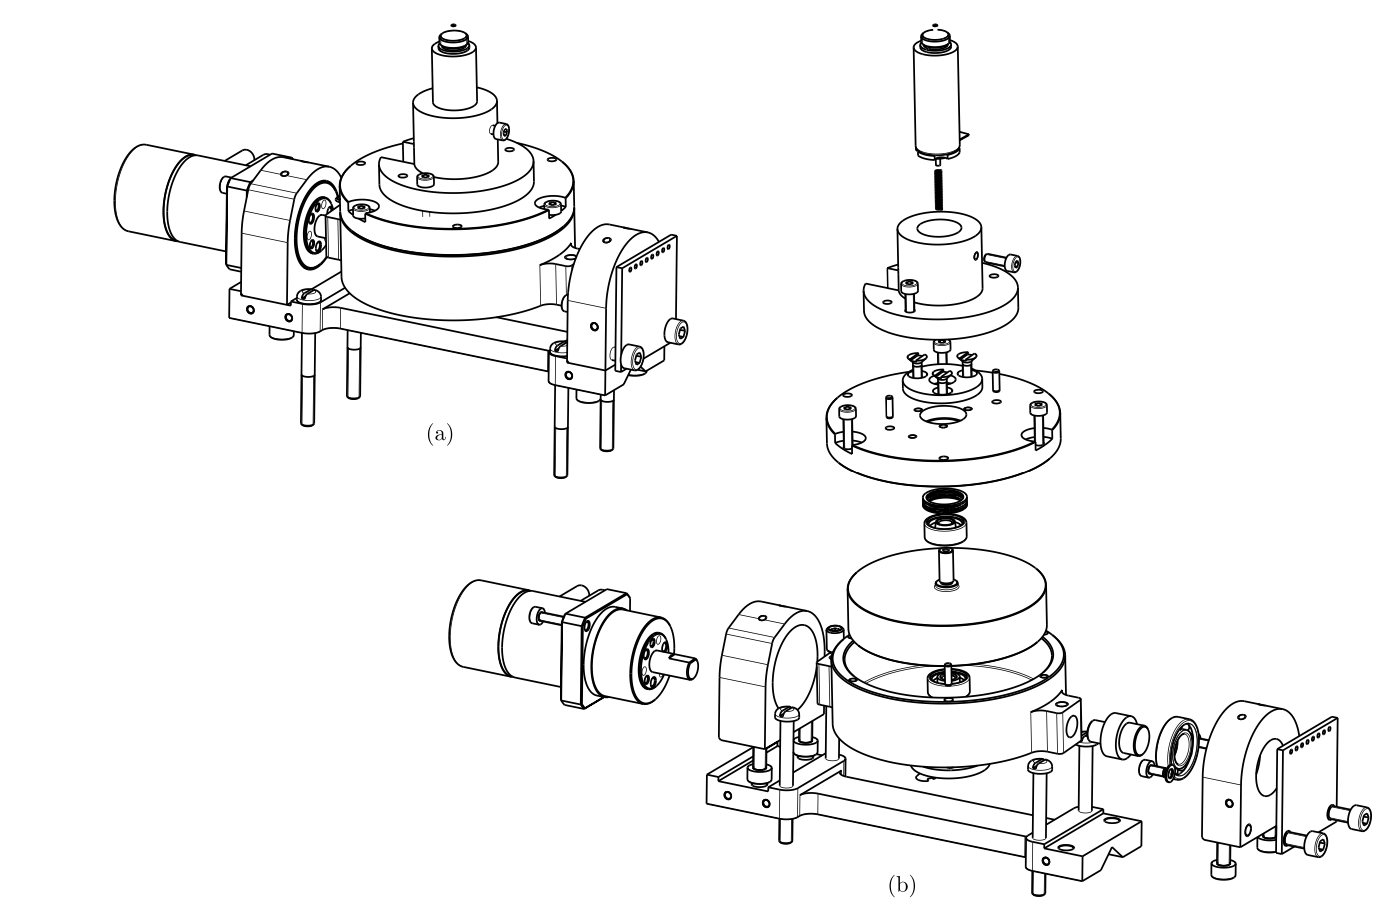
\includegraphics[width=0.6\linewidth]{img/fig19}
\caption{Vues d’ensemble du modèle GyroLock (a) vue générale de l’assemblage (b) vue éclatée}
\label{fig19}
\end{center}
\end{figure}

Une simulation statique par éléments finis nous permet d’obtenir des informations sur la répartition des contraintes subies par la pièce.

\paragraph{Hypothèse:} le matériau doit avoir une limite d’élasticité $ R_{p0,2}$ à $0,2\%$ de déformation plastique telle que $\sigma_{max}\leq \frac{ R_{p0,2}}{s}$ avec s un coefficient de sécurité, qui vaut $s=3$ pour notre système.

\begin{figure}[ht]
\begin{center}
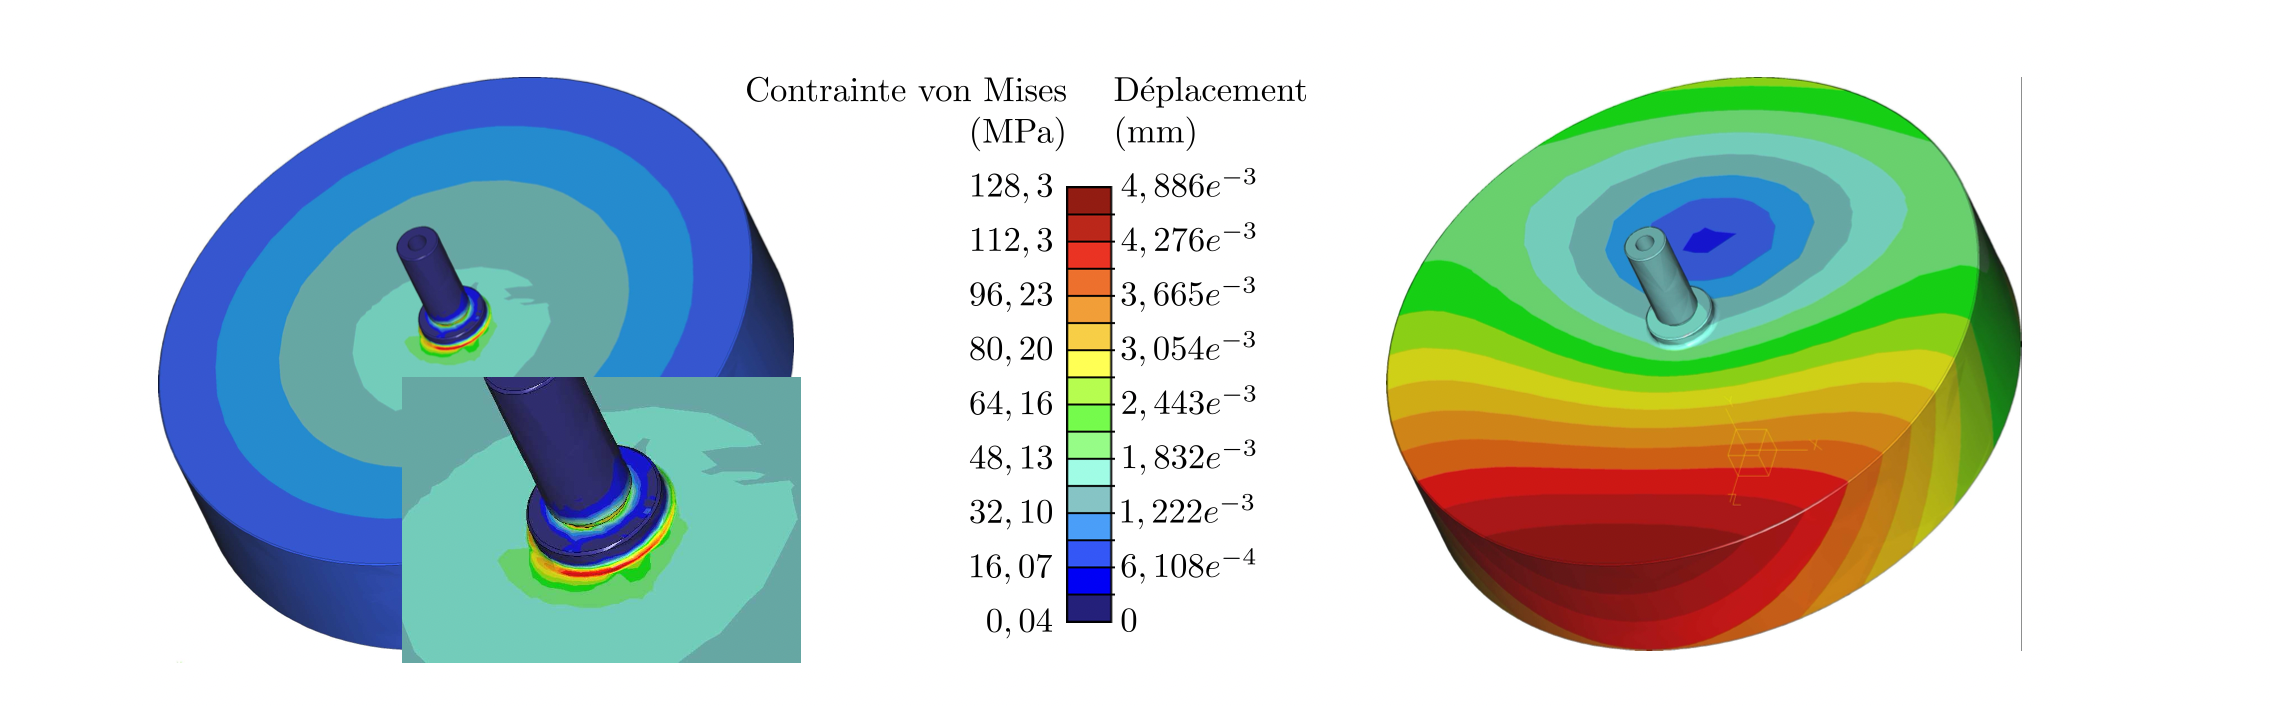
\includegraphics[width=0.6\linewidth]{img/fig20}
\caption{Contraintes et déplacement du gyroscope soumis à la force centrifuge et au couple gyroscopique maximal (figure donnée en annexe en couleur)}
\label{fig20}
\end{center}
\end{figure}

\question{En utilisant la figure \ref{fig20}, donner la valeur de contrainte maximale que peut subir la toupie  $\sigma_{max}$. En déduire la valeur de $R_{p0,2}$ que le matériau doit avoir pour respecter le cahier des charges.}

~\

Les figures \ref{fig21} et \ref{fig22} donnent les caractéristiques des 2 matériaux suivants: Alliage de titane Ti6 Al4 V et Acier inoxydable 316L (X2CrNiMo17-12-2).

\begin{figure}[ht]
\begin{center}
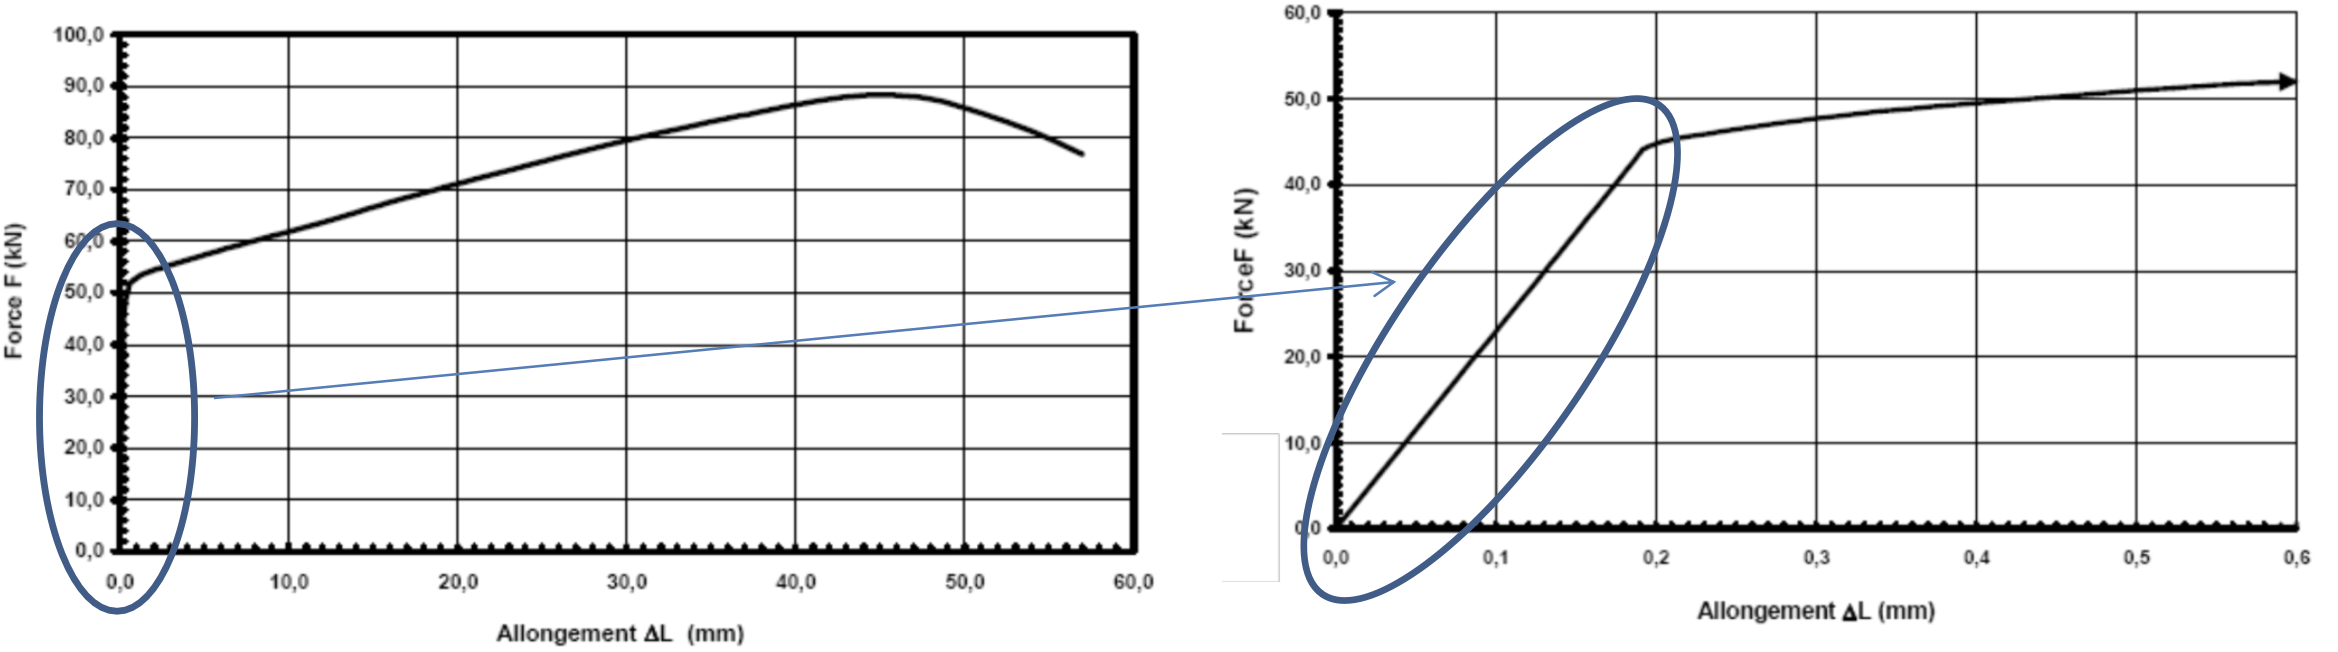
\includegraphics[width=0.75\linewidth]{img/fig21}
\caption{Courbe conventionnelle de traction acier 316L $F=f(\Delta l)$ (éprouvette $D_0=15\;mm$ et $L0=150\;mm$)}
\label{fig21}
\end{center}
\end{figure}

\begin{figure}[ht]
\begin{center}
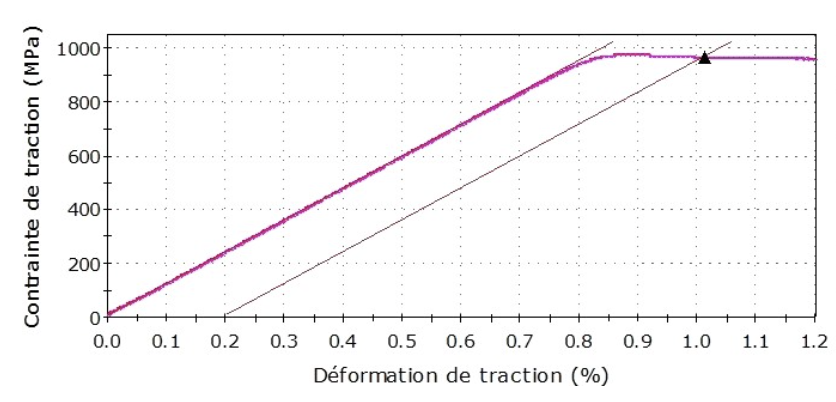
\includegraphics[width=0.55\linewidth]{img/fig22}
\caption{Courbe traction alliage titane Ti Al4 V}
\label{fig22}
\end{center}
\end{figure}

\begin{table}
\begin{tabularx}{\textwidth}{|l|l|X|X|X|}
\hline
Données matériaux & Prix (€/kg) & Tenue à la corrosion & Température de fusion (°C) & $\rho$ (Masse volumique) ($kg\cdot m^{-3}$)\\
\hline
Acier inoxydable 316 L & 5.9 & + & 1230-1530& 7800 \\
\hline
Alliage Titane & 30 & +++ & 1650-1670 & 4500 \\
\hline
\end{tabularx}
\caption{Caractéristiques des deux matériaux}
\label{tab1}
\end{table}

%\paragraph{Dureté:}

%Alors que la dureté Brinell de l'acier inoxydable varie considérablement avec la composition de l'alliage et le traitement thermique, il est dans la plupart des cas plus dur que le titane. Cependant, le titane se déforme facilement lorsqu'il est rayé. Afin d'éviter cela, le titane forme une couche d'oxyde appelée couche d'oxyde de titane qui forme une surface exceptionnellement dure qui résiste à la plupart des forces de pénétration. Le titane et l'acier inoxydable sont tous deux des matériaux résistants qui fonctionnent très bien lorsqu'ils sont exposés à des environnements bruts et difficiles.

\question{Donner la valeur de $R_{p0,2}$ pour chacun des matériaux à partir de la courbe conventionnelle de traction.}

\question{A partir de ces résultats et du tableau \ref{tab1}, en justifiant, donner le choix de matériau final pour la toupie d’un point de vue résistance.}

\question{Citer un procédé d’obtention pour cette toupie.}

\section{Conception}

La toupie est en liaison pivot avec l’étrier.

Cette liaison est réalisée à partir des roulement à bille à contact oblique présentés sur la figure \ref{fig23} montés en X. Afin d'ajouter de la souplesse au montage, un des appuis sera réalisé par un ressort présent sur le dessin du document réponse.

\begin{figure}[ht]
\begin{center}
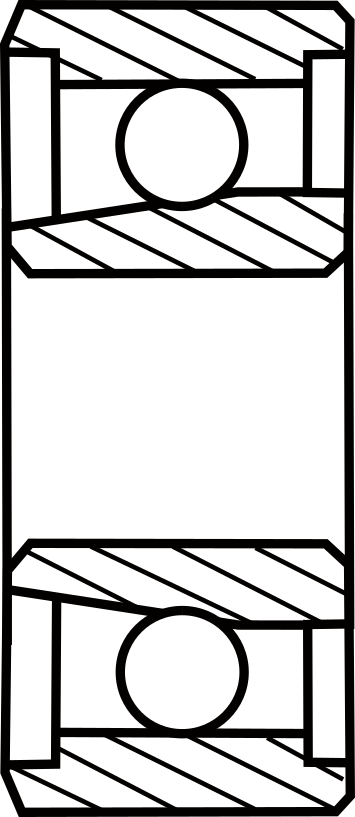
\includegraphics[width=0.1\linewidth]{img/fig23}
\caption{Roulement à bille à contact oblique}
\label{fig23}
\end{center}
\end{figure}

\newpage

\begin{figure}[ht]
\begin{center}
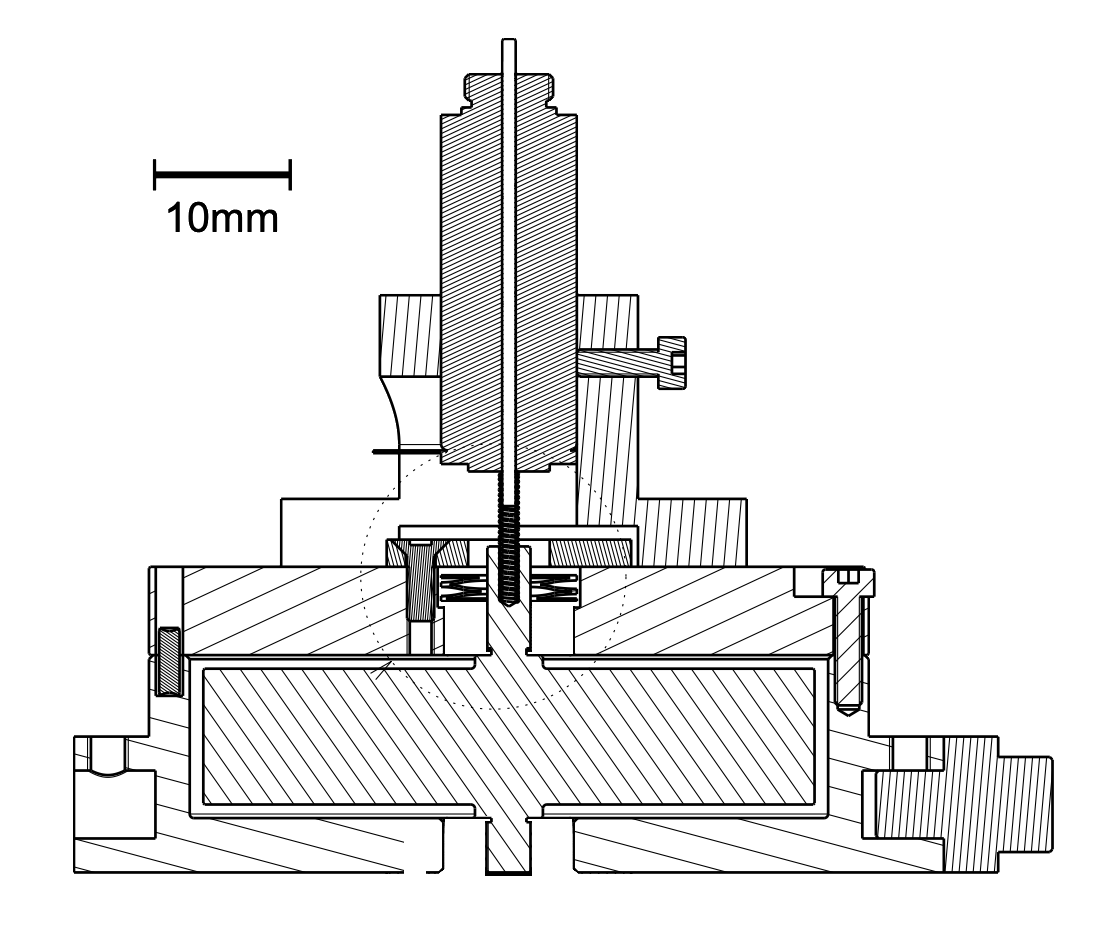
\includegraphics[width=0.8\linewidth]{img/fig24}
\caption{Montage de la toupie à compléter sur le zoom du document réponse}
\label{fig24}
\end{center}
\end{figure}

\question{Compléter la conception du document réponse afin d'implanter les roulements et les pièces nécessaires à leurs arrêts axiaux.}

\newpage

~\

\cleardoublepage

\newpage

\cleardoublepage

%\def\public

\ifdef{\public}{\pagestyle{docreponse}}{\pagestyle{correction}}

\ifdef{\public}{
\begin{tikzpicture} 
	\draw (0,0) rectangle (2,2);
	\draw (0,0) -- (2,2);
	\draw (1.5,0.5) node {\large 20};
	\draw (2.5,0) rectangle (16,2);
	\draw (4.2,1.7) node {\large Commentaires:};
\end{tikzpicture}\\} 


%1
\reponse{9}{}{Direction dorso-ventrale : déplacement maximal du point $P$ $u_d^{\text{max}} \approx 3,7$mm et $u_d^{\text{min}} \approx -2,5$mm.\\

Dans le plan frontal, $u_f^{\text{max}} \approx 0,25$mm et $u_f^{\text{min}} \approx -0,4$mm.\\

Comme le déplacement dorso-ventral est supérieur à $2$mm, il faut une stabilisation active.}

%2
\reponse{9}{}{On a $\overrightarrow{P_0P} = \overrightarrow{P_0 O_0} + \overrightarrow{O_0 P} = L \overrightarrow{z_1} - L \overrightarrow{z_0}$.

Avec :\\
$$ \overrightarrow{z_1} = \cos(\theta_{1y})\overrightarrow{z_{1'}} + \sin(\theta_{1y})\overrightarrow{x_{1'}} = \cos(\theta_{1y})\cos(\theta_{1x})\overrightarrow{z_0} - \cos(\theta_{1y})\sin(\theta_{1x})\overrightarrow{y_0} + \sin(\theta_{1y})\overrightarrow{x_0}$$

Ainsi:

$$ \overrightarrow{P_0P} = L\left[ \sin(\theta_{1y})\overrightarrow{x_0} - \cos(\theta_{1y})\sin(\theta_{1x})\overrightarrow{y_0} + \left( \cos(\theta_{1y})\cos(\theta_{1x}) - 1 \right)\overrightarrow{z_0} \right] $$

Donc :

$$u_d = \overrightarrow{P_0P}\cdot \overrightarrow{y}_0 = -L \cos(\theta_{1y})\sin(\theta_{1x})$$

$$u_f = \left\|\overrightarrow{P_0P}-u_d\overrightarrow{y}_0\right\| = L\sqrt{\sin^2(\theta_{1y}) + \left( \cos(\theta_{1y})\cos(\theta_{1x}) - 1 \right)^2}$$}

%3
\reponse{9}{}{On prend $\cos(\theta_{i}) \approx 1$ et $\sin(\theta_{i}) \approx \theta_{i}$ pour $\theta_i = \theta_{1x}$ ou $\theta_i = \theta_{1y}$.\\

Par conséquent $\overrightarrow{P_0P} \approx L\left[ \theta_{1y}\overrightarrow{x}_0 - \theta_{1x}\overrightarrow{y}_0 \right]$ donc: $u_d \approx -L \theta_{1x}$ et $u_f \approx L|\theta_{1y}|$

En s'appuyant sur la question 1:

$$ \Delta \theta_{1x} = \dfrac{u_d^{\text{min}} - u_d^{\text{max}}}{L} \approx \dfrac{-2,3 - 3,5}{0,3\cdot 10^{3}} \approx -1,9\cdot 10^{-2}\text{rad}$$

$$\Delta \theta_{1y} = \dfrac{u_f^{\text{max}} - u_f^{\text{min}}}{L} \approx \dfrac{0,25 + 0,4}{0,3\cdot 10^{3}} \approx 2,1\cdot 10^{-3}\text{rad} $$

On a $\dfrac{\Delta\theta_{1x}}{\Delta\theta_{1y}}=10$, donc la rotation autour de $(O_0,\overrightarrow{y_1})$ négligeable par rapport à $(O_0,\overrightarrow{x_0})$.

Si la rotation $(O_0,\overrightarrow{z_0})$ est négligée, alors on peut considérer la liaison comme une pivot autour de $(O_0,\overrightarrow{x_0})$.}

%4
\reponse{2}{}{On veut compenser les mouvements dans la direction dorso-ventrale ($\left( O_0,\overrightarrow{x}_0 \right)$), donc il faut un moment selon cet axe.}

%5
\reponse{0}{\begin{center}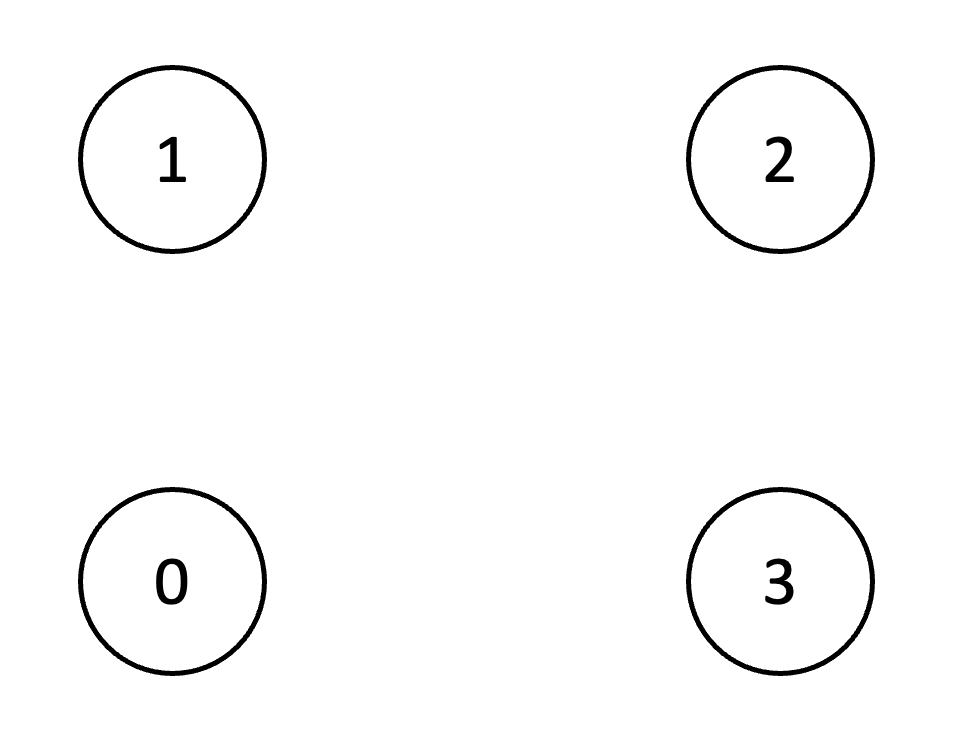
\includegraphics[width=0.6\linewidth]{img/dr05}\end{center}}{\begin{center}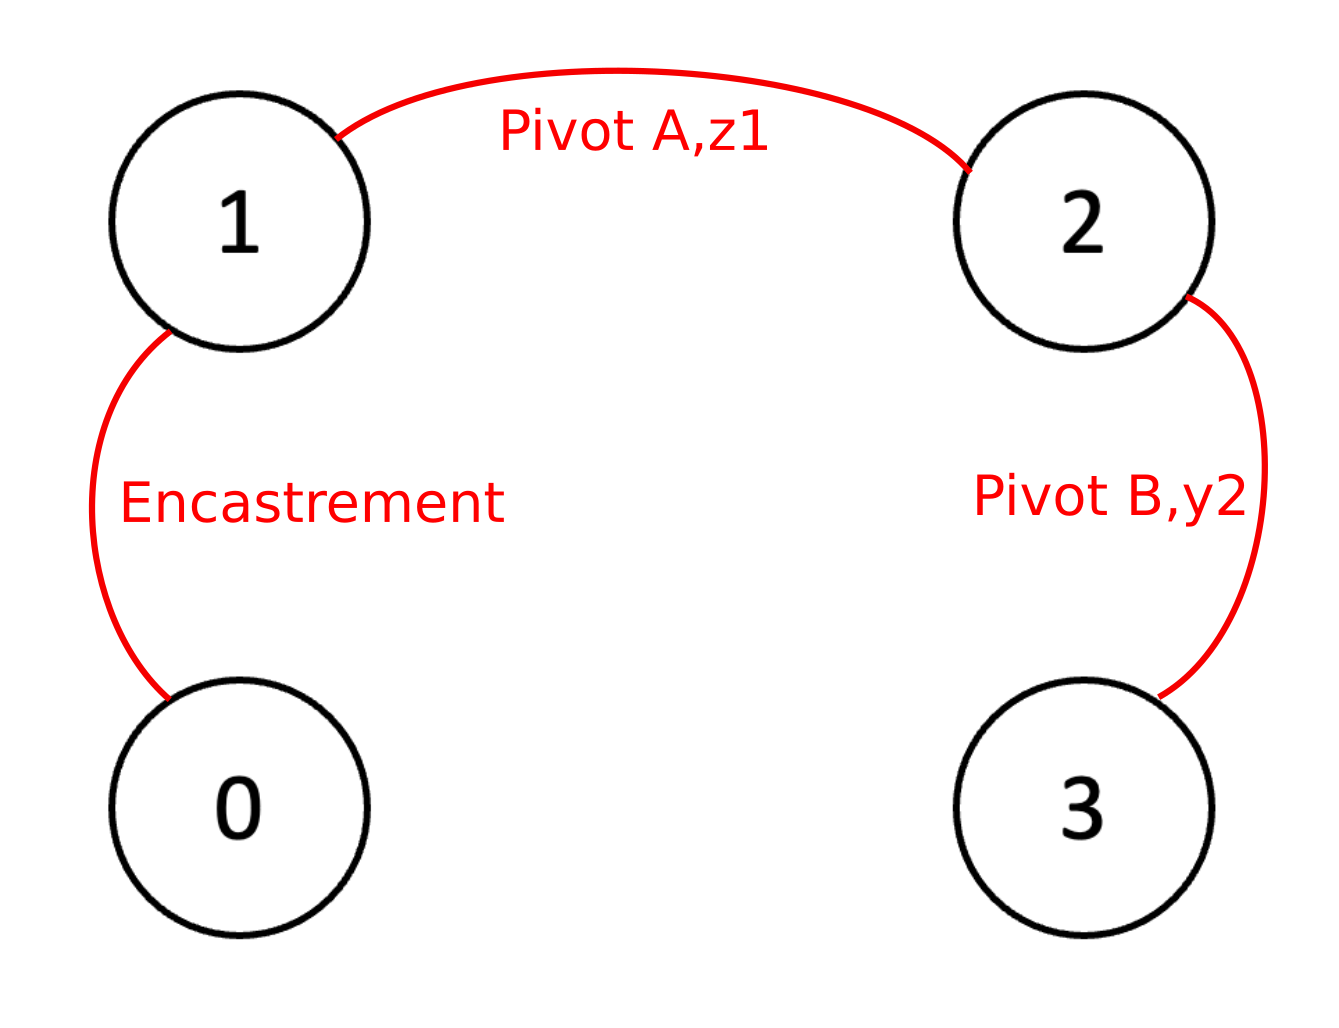
\includegraphics[width=0.6\linewidth]{img/dr05_cor}\end{center}}

\ifdef{\public}{\newpage}{}

%6
\reponse{5}{}{Bilan des Actions Mécaniques:
\begin{itemize}
 \item $0\rightarrow 1$ (encastrement).
\end{itemize}}

%7
\reponse{4}{}{$\Sigma\overrightarrow{M}(G_3,ext \rightarrow \Sigma)=\overrightarrow{M}(G_3,0 \rightarrow 1)=L_{01}\cdot\overrightarrow{x_1}+M_{01}\cdot\overrightarrow{y_1}+N_{01}\cdot\overrightarrow{z_1}$.}

%8
\reponse{9}{}{$\overrightarrow{M}(G_3,3/0)=\left(\dfrac{d}{dt}\left(B_3\dot{\theta}_3\overrightarrow{y_2}+A_3\dot{\theta}_2\overrightarrow{z_2}\right)\right]$, or $\left[\dfrac{d\overrightarrow{y_2}}{dt}\right]_{B_0}=-\dot{\theta}_2\cdot\overrightarrow{x_2}$ et $\left[\dfrac{d\overrightarrow{z_2}}{dt}\right]_{B_0}=\overrightarrow{0}$

Donc, $\overrightarrow{\delta}(G_3,3/0)=-B_3\dot{\theta}_3\dot{\theta}_2\overrightarrow{x_2}+B_3\ddot{\theta}_3\overrightarrow{y_2}+A_3\ddots\theta}_2\overrightarrow{z_2}$}

\ifdef{\public}{\newpage}{}

%9
\reponse{9}{}{$\overrightarrow{x_2}=cos\theta_2\overrightarrow{x_1}+sin\theta_2\overrightarrow{y_1}$ et $\overrightarrow{y_2}=-sin\theta_2\overrightarrow{x_1}+cos\theta_2\overrightarrow{y_1}$
$\overrightarrow{\delta}(G_3,3/0)=B_3\left(-\dot{\theta}_3\dot{\theta}_2\cos\theta_2-\ddot{\theta}_3\sin\theta_2\right)\overrightarrow{x_1}+B_3\left(-\dot{\theta}_3\dot{\theta}_2\sin\theta_2+\ddot{\theta}_3\cos\theta_2\right)\overrightarrow{y_1}+A_3\ddot{\theta}_2\overrightarrow{z_1}$
$L_{01}(t)=-B_3\left(\dot{\theta}_3\dot{\theta}_2\cos\theta_2+\ddot{\theta}_3\sin\theta_2\right)$\\
$M_{01}(t)=B_3\left(-\dot{\theta}_3\dot{\theta}_2\sin\theta_2+\ddot{\theta}_3\cos\theta_2\right)$\\
$N_{01}(t)=A_3\ddot{\theta}_2$.
}


%10
\reponse{12}{}{Avec $\ddot{\theta}_3=0$, car $\dot{\theta}_3=cst$ et en ajoutant $\overrightarrow{M}(G_3,c\rightarrow 1)=\overrightarrow{G_3P}\wedge \overrightarrow{R_{c\rightarrow 1}}=-f_c(L-L_{G_3}).\overrightarrow{x_1}$.

Ainsi le système précédent devient:\\
$L_{01}(t)-f_c(L-L_{G_3})=-B_3\dot{\theta}_3\dot{\theta}_2\cos\theta_2$\\
$M_{01}(t)=-B_3\dot{\theta}_3\dot{\theta}_2\sin\theta_2$\\
$N_{01}(t)=A_3\ddot{\theta}_2$.

Pour avoir $L_{01}(t)=0$, il faut $f_c(L-L_{G_3})=K_3\dot{\theta}_2\cos\theta_2$

Donc, $\dot{\theta}_2=\dfrac{f_c(L-L_{G_3})}{K_3\cos\theta_2}$}

%11
\reponse{3}{}{Si on veut $M_{01}(t)$ faible, alors $\sin\theta_2(t)$ doit être faible.\\Si on veut $N_{01}(t)$ faible, alors $\ddot{\theta}_2(t)$ doit être faible.}

%12
\reponse{5}{}{Une demi-période, $\dfrac{1}{2}T=\dfrac{1}{2}\dfrac{1}{f}=\dfrac{1}{2}\dfrac{2}{3}\approx 0,33s$.

Le temps de réponse $t_{r5\%}\approx0,02$ donc c'est bon.

$H_2(p) = \dfrac{\Omega_2(p)}{\Omega_{c2}(p)} = K_2 = 1$.}

%13
\reponse{6}{}{Avec $\theta^*_2(p) = 0$

$$ \Omega_{c2}(p) = U(p) - C(p)\cdot \dfrac{K_2}{p}\Omega_{c2}(p) $$

Or $\Omega_{c2}(p) = \dfrac{p}{K_2}\theta_2(p)$ donc:

$$H_{\theta_2}(p) = \dfrac{K_2}{p + K_2 C(p)}$$}

%14
\reponse{4}{}{Correction proportionnelle: $\displaystyle\lim_{t\to +\infty}\theta_2(t) = \lim_{p\to 0}p\theta_2(p) = \lim_{p\to 0} p\cdot H_{\theta_2}(p)\dfrac{1}{p} = \dfrac{1}{K_{10}}$}

%15
\reponse{4}{}{Correction proportionnelle-intégrale: $\displaystyle\lim_{t\to +\infty}\theta_2(t) = \lim_{p\to 0}p\theta_2(p) = \lim_{p\to 0}\dfrac{K_2 p}{p^2 + K_2K_{10}p + K_2K_{11}} = 0$}

%16
\reponse{4}{}{La dérive de l'étrier sera évitée avec la correction proportionnelle-intégrale.}

%17
\reponse{4}{}{$$ H_{m}(p) = \dfrac{H_2(p)}{1+ H_2(p)\dfrac{C(p)}{p}} = \dfrac{\dfrac{1}{K_{11}}p^2}{1 + \dfrac{K_{10}}{K_{11}}p + \dfrac{p^2}{K_2K_{11}}} $$}

%18
\reponse{5}{}{On peut identifier:

$$ \omega_m = \sqrt{K_2 K_{11}} \quad ; \quad \xi_m = \dfrac{1}{2}K_{10}\sqrt{\dfrac{K_{2}}{K_{11}}} $$

Comme $K_2 = 1$, on calcule:

$K_{11} = \dfrac{\omega_m^2}{K_2} = 6,00\text{rad}^2.\text{s}^{-2}$ et $K_{10} = \dfrac{2\xi_m}{\omega_m}K_{11} = 1,81\text{rad}.\text{s}^{-1}$
}

\ifdef{\public}{\newpage}{}

%19
\reponse{6}{}{D'après le schéma-bloc, $\dfrac{Y(p)}{H_1(p)} = C_x(p) - H_{\text{pert}}(p)F_c(p)$.

On a $Y(p) = L \theta_1(p)$), donc l'équation précédente devient :

$$ \left( J_x p^2 + f p + k \right)\dfrac{Y(p)}{L} = C_x(p) - L F_c(p) $$

Donc $H_1(p) = \dfrac{L}{J_x p^2 + f p + k}$ et $H_{\text{pert}}(p) = L$.
}

%20
\reponse{6}{}{$H_1(p) = \dfrac{\dfrac{L}{k}}{1 + \dfrac{f}{k}p + \dfrac{J_x}{k}p^2}$.

Donc :
\begin{itemize}
\item $K_1 = \dfrac{L}{k} = \dfrac{0,3}{95} = 3,2\cdot 10^{-3}$rad/N
\item $\omega_1 = \sqrt{\dfrac{k}{J_x}} = \sqrt{\dfrac{95}{1,14\cdot 10^{-2}}} = 91,3$rad/s
\item $\xi_1 = \dfrac{1}{2}\cdot \dfrac{f}{\sqrt{k J_x}} = \dfrac{1}{2}\cdot \dfrac{64\cdot 10^{-3}}{\sqrt{95 \times 1,14\cdot 10^{-2}}} = 0,03$. 
\end{itemize} 
}

%21
\reponse{0}{\begin{center}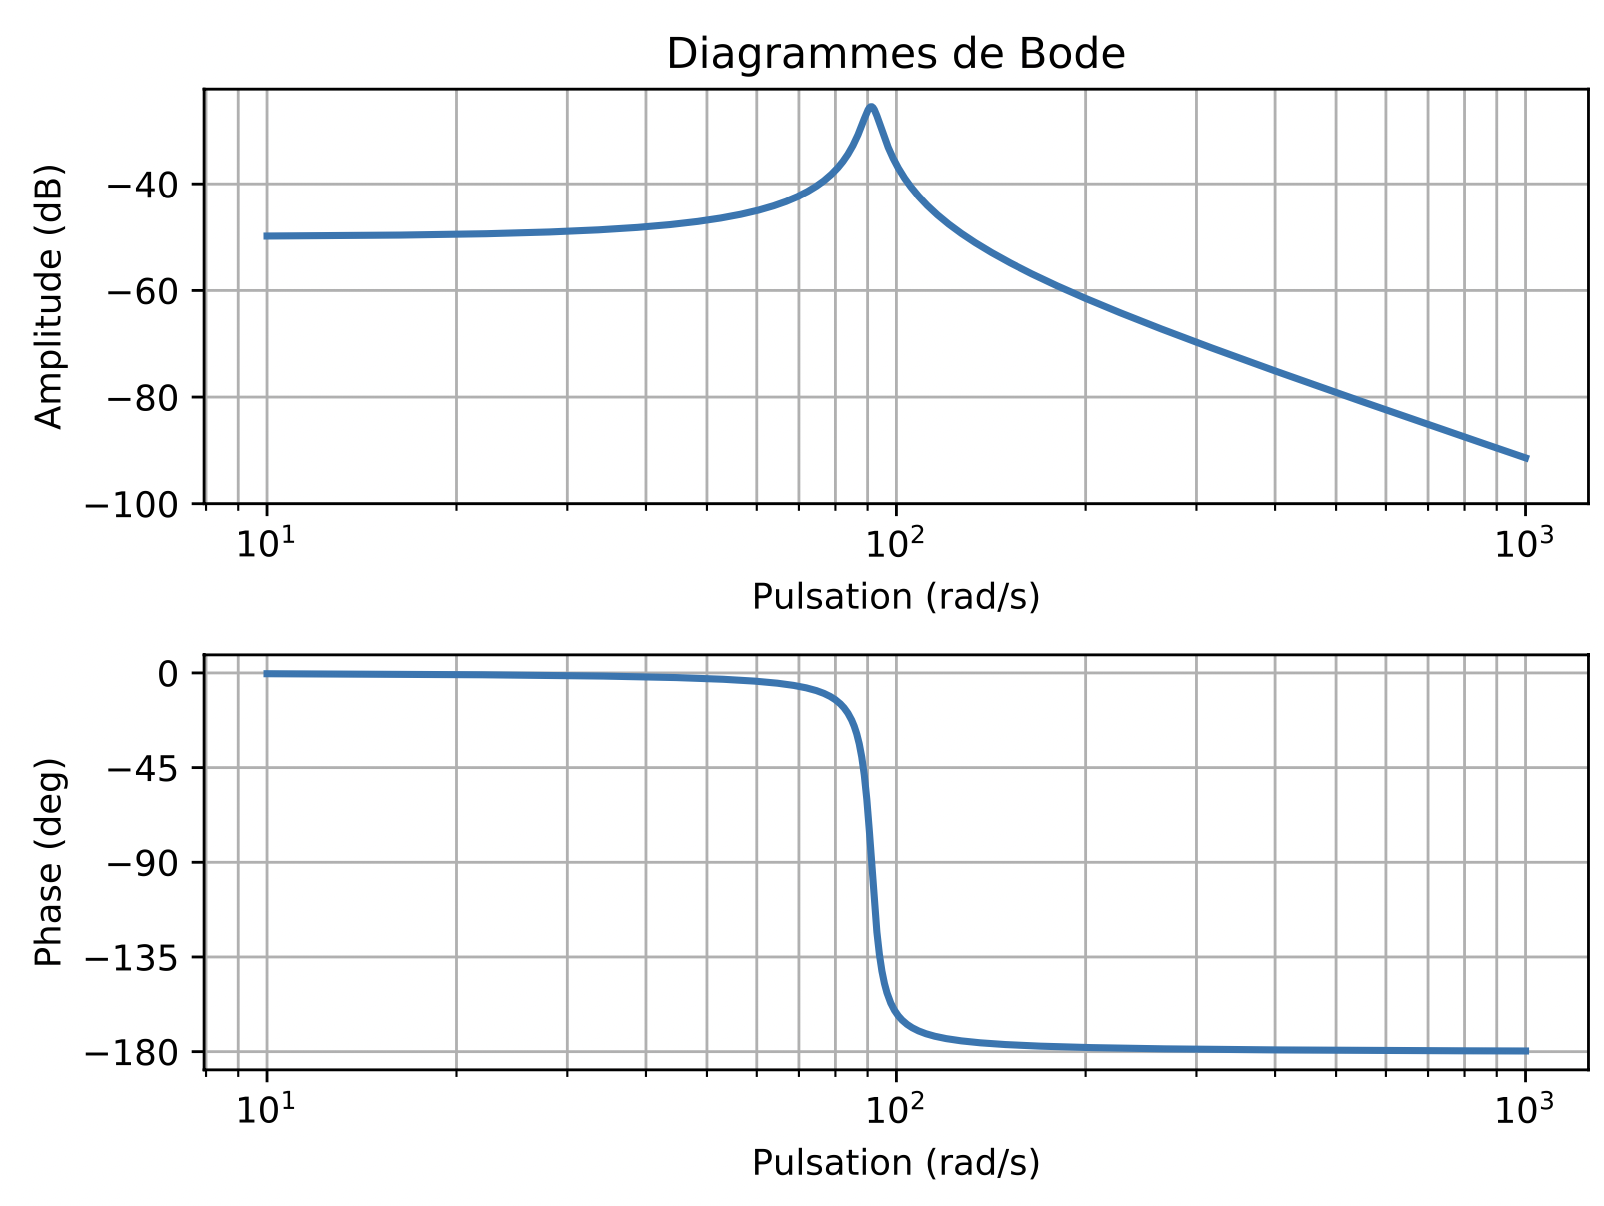
\includegraphics[width=0.6\linewidth]{img/dr21}\end{center}}{\begin{center}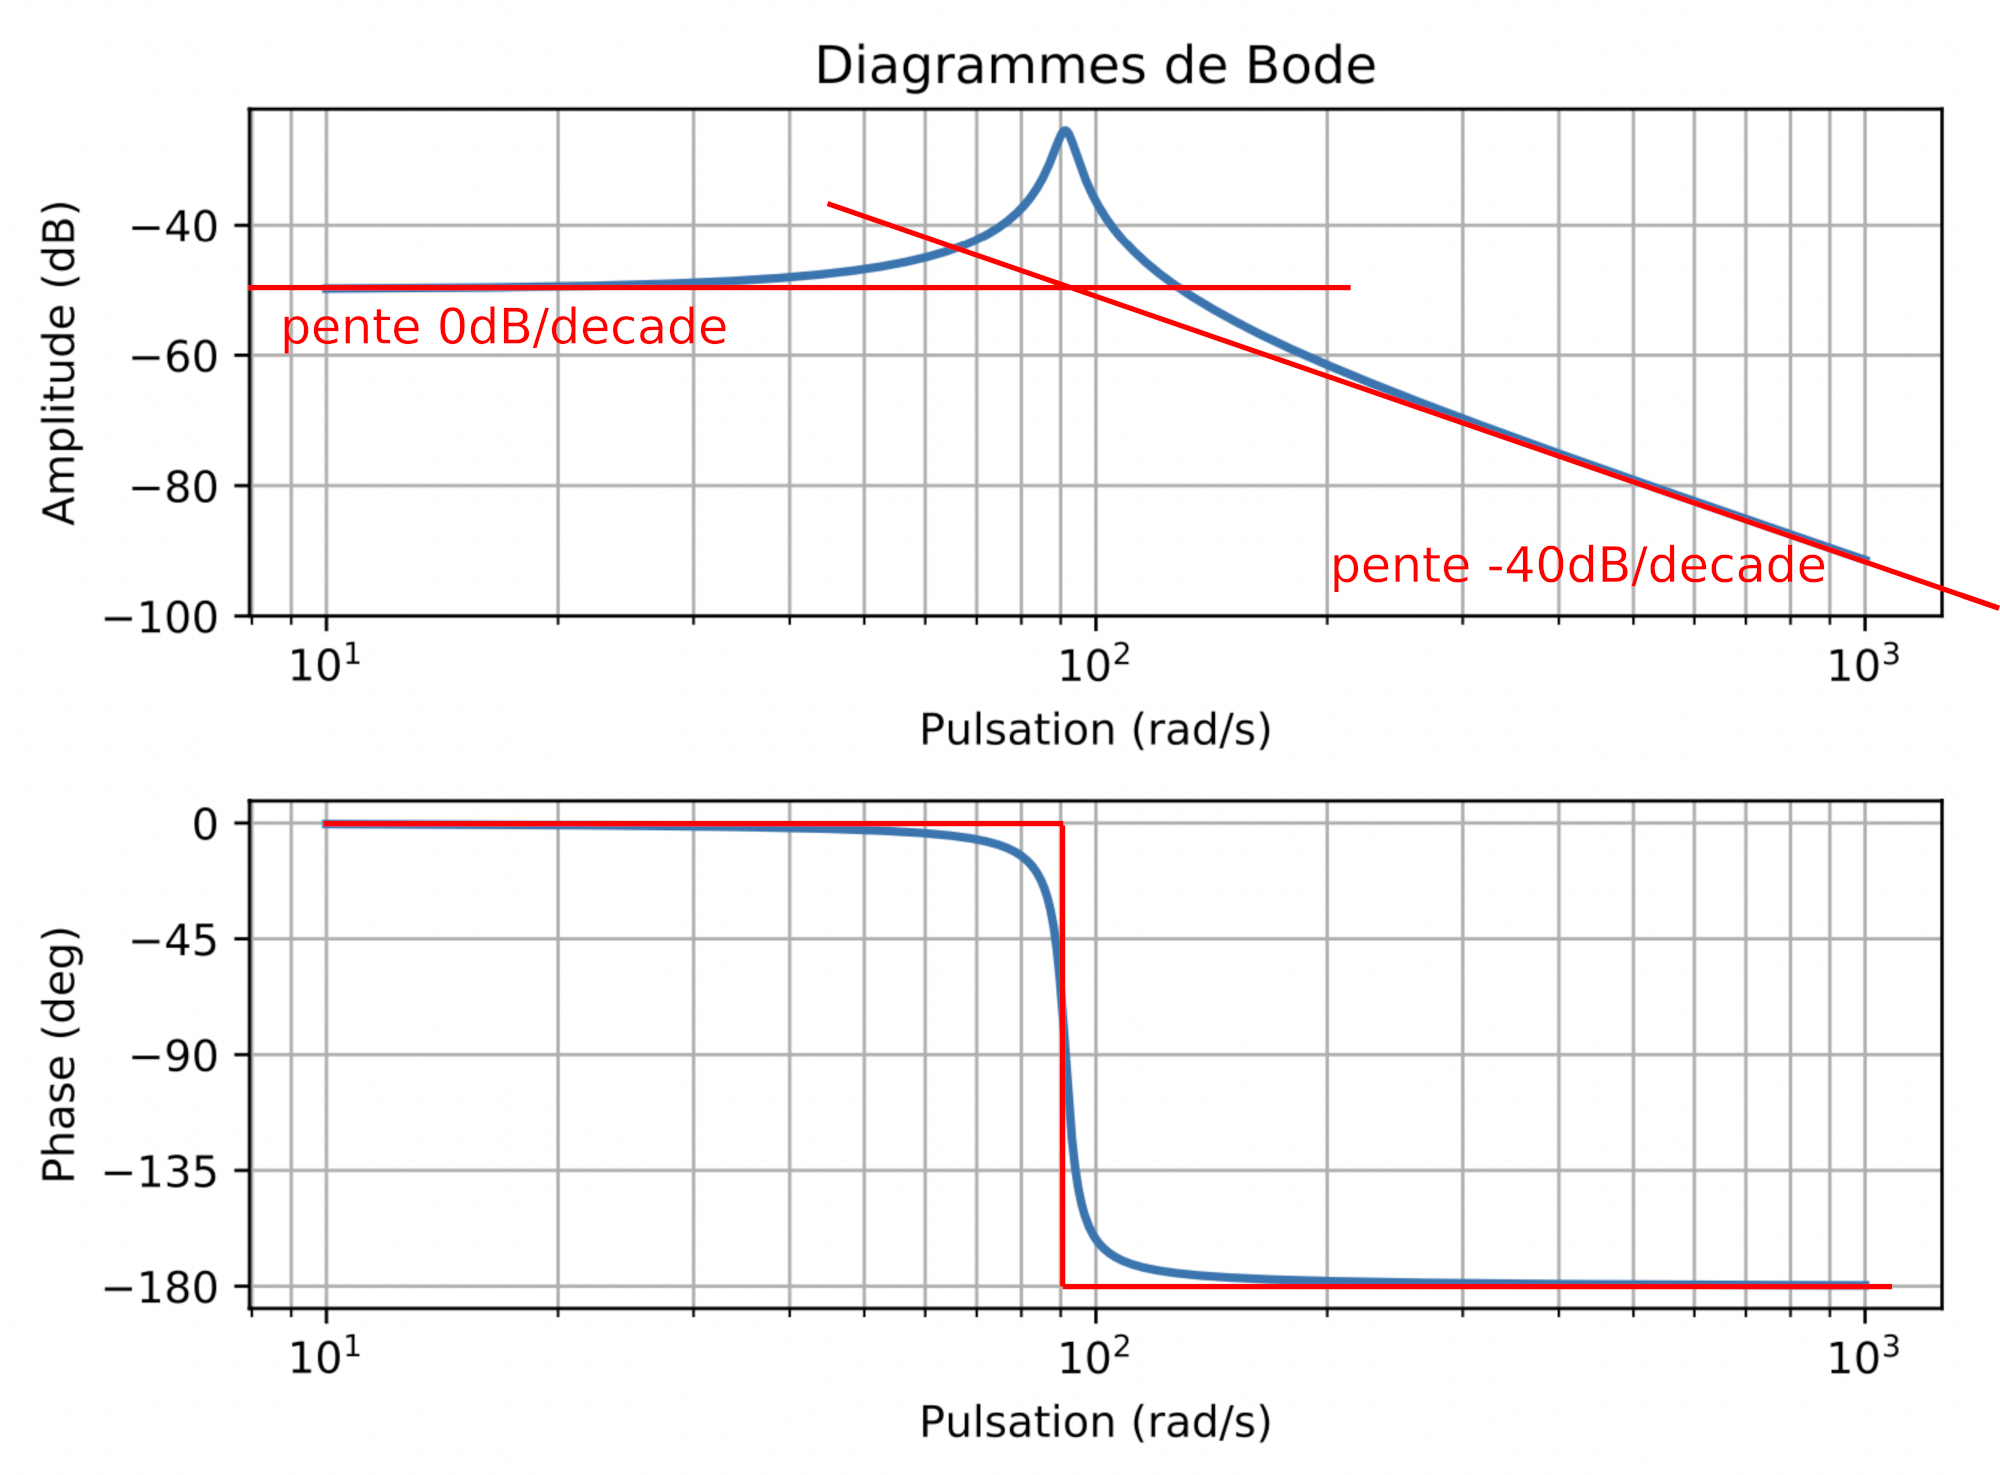
\includegraphics[width=0.6\linewidth]{img/dr21_cor}\end{center}

$\omega_0=90rad\cdot s^{-1}$

$\frac{\left| H(j\omega)_{max} \right|}{\left| H(0) \right|}=10^{\frac{30}{20}}=10^{1.5}\approx 30$
}

\ifdef{\public}{\newpage}{}

%22
\reponse{3}{}{Déplacement maximal de 2mm par rapport à la référence, donc le cela respecte le cahier des charges.}

%23
\reponse{4}{}{$\sigma_{max}=128,3MPa$

$\sigma_{max}\leq \frac{Re}{S}$, $Re\geq 384,9MPa$.}

%24
\reponse{0}{\begin{center}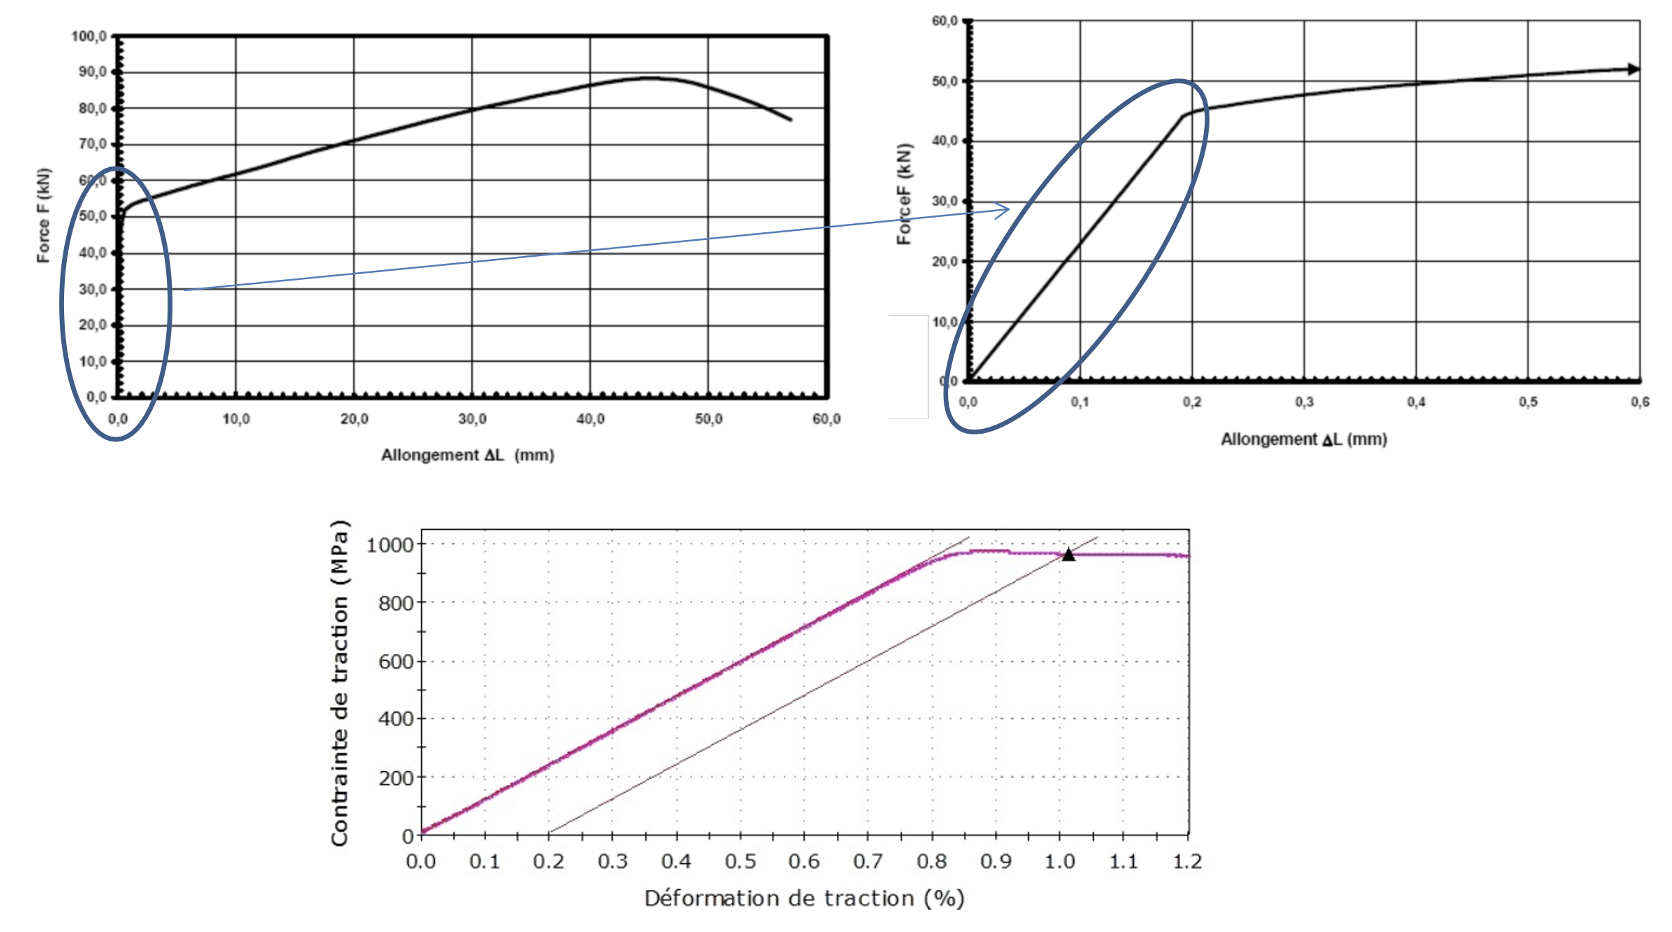
\includegraphics[width=\linewidth]{img/dr24}\end{center}}{\begin{center}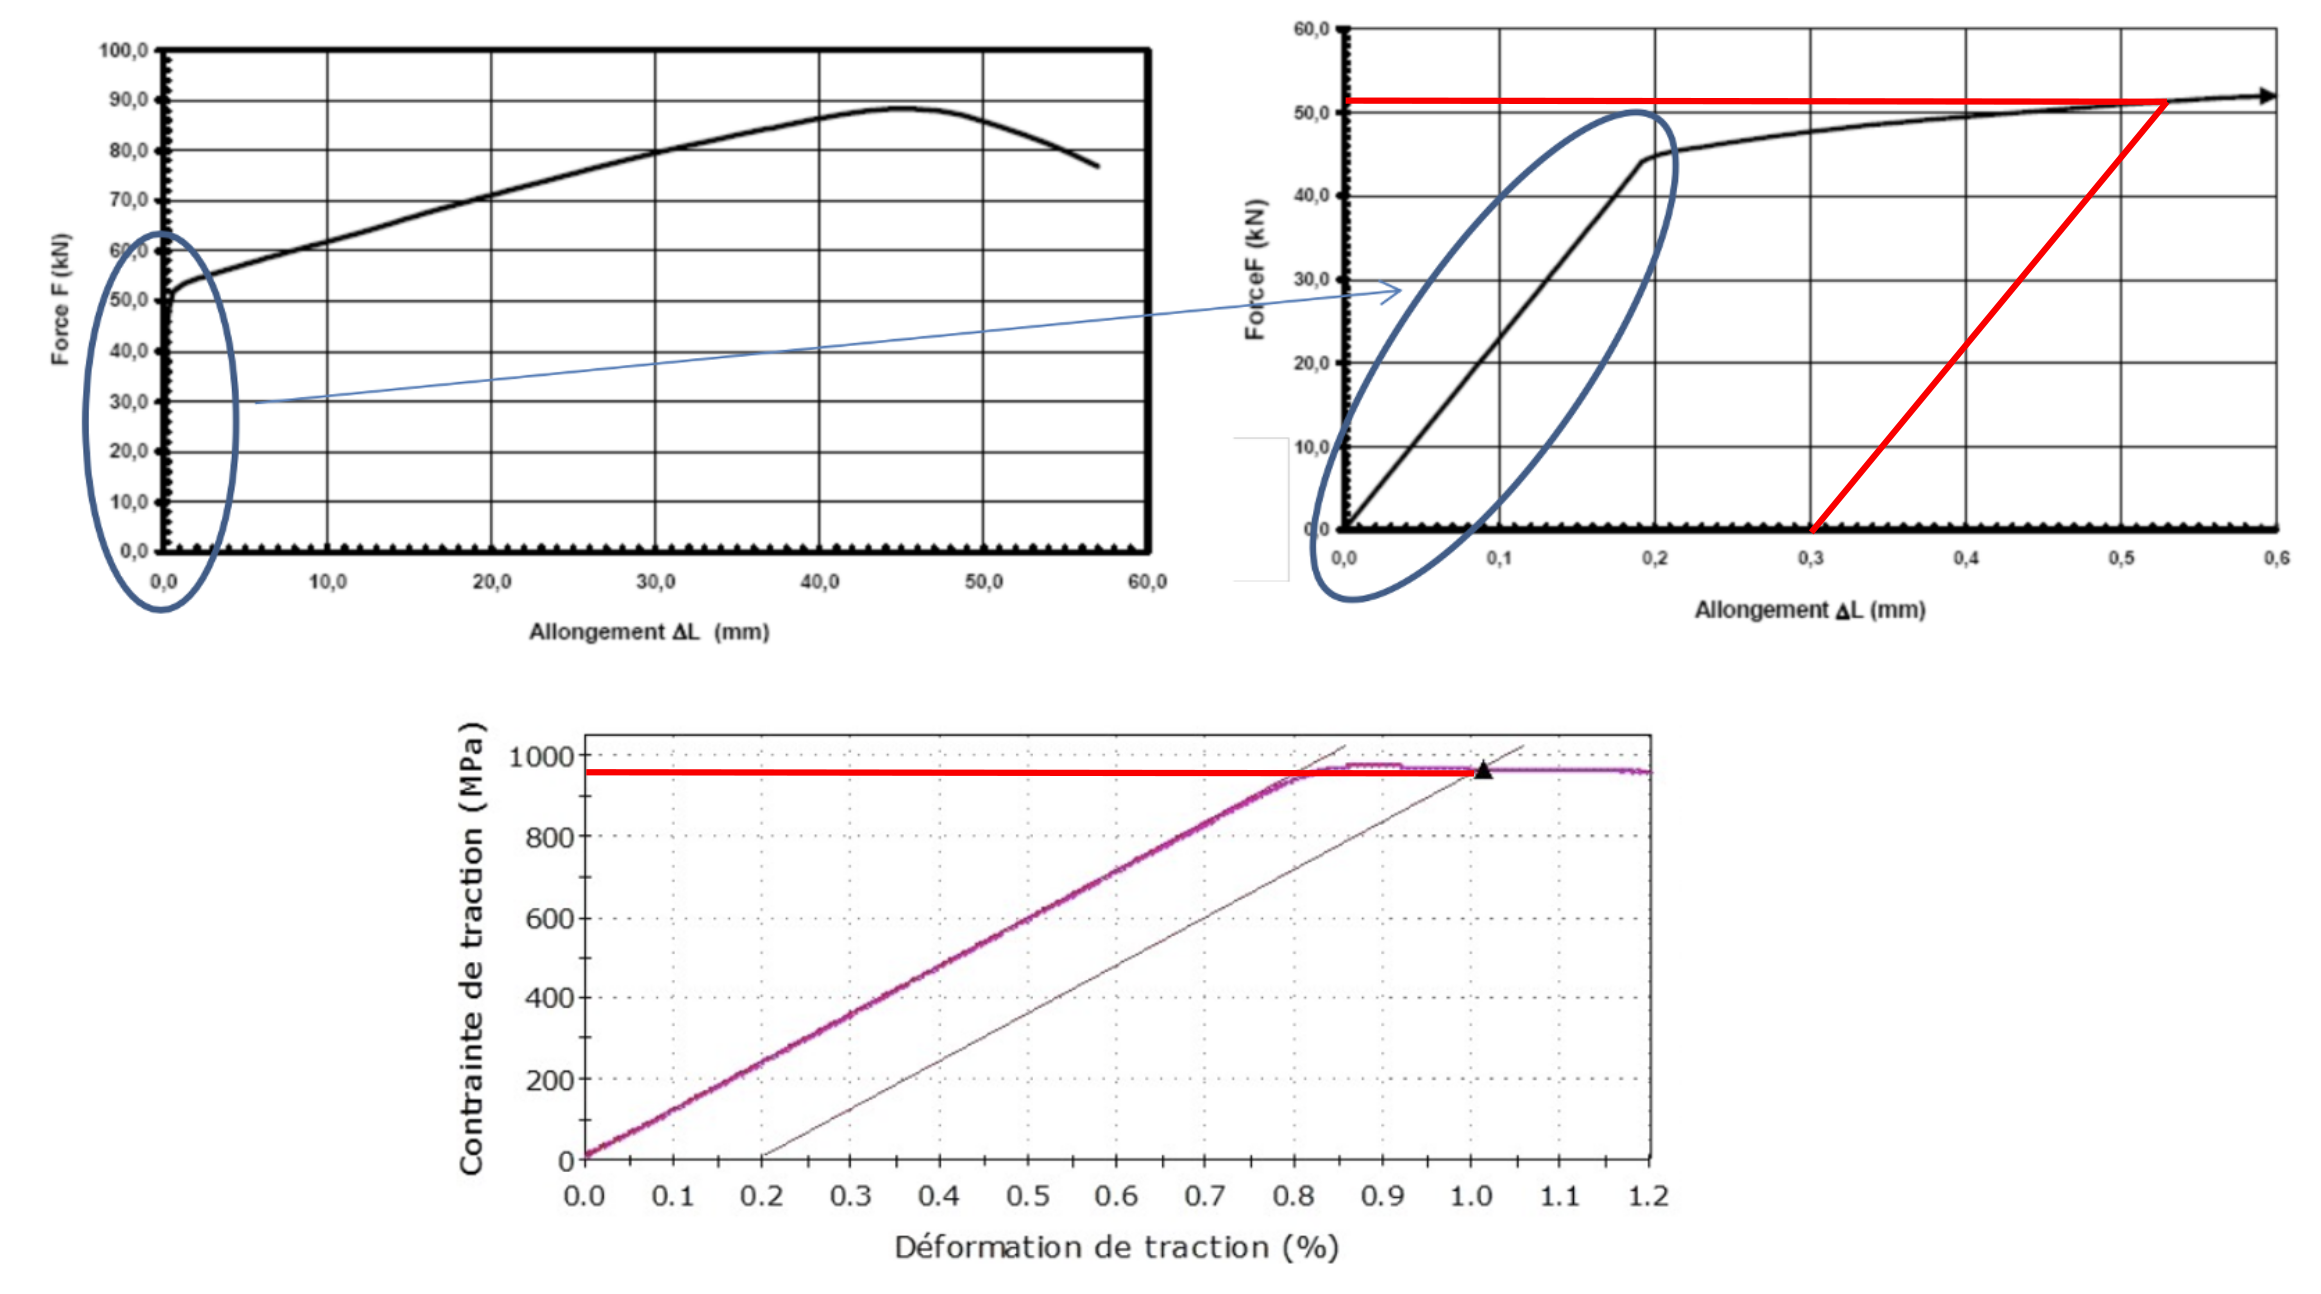
\includegraphics[width=\linewidth]{img/dr24_cor}\end{center}

Pour l'acier : $0,2\%150mm=0,3mm$, ce qui donne $F_{0,2}=50kN$, donc $R_{p0,2\%}=\dfrac{50\cdot 1000}{7,5^2\cdot\pi}\approx\dfrac{50\cdot 1000}{175}\approx\dfrac{10000}{35}\approx300MPa$

Pour le titane : on lit directement $R_{p0,2\%}=900MPa$.
}

\ifdef{\public}{\newpage}{}

%25
\reponse{3}{}{D'après les résultats le matériau le plus adapté est le titane.}

%26
\reponse{2}{}{Cette toupie peut être moulée puis usinée.}

%27
\reponse{0}{\begin{center}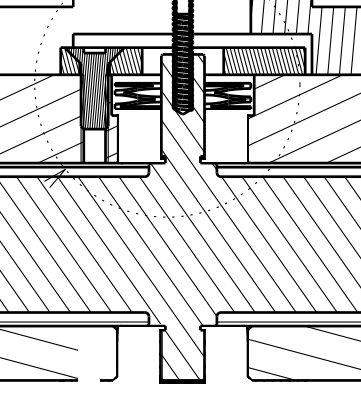
\includegraphics[width=0.7\linewidth]{img/dr27}\end{center}}{\begin{center}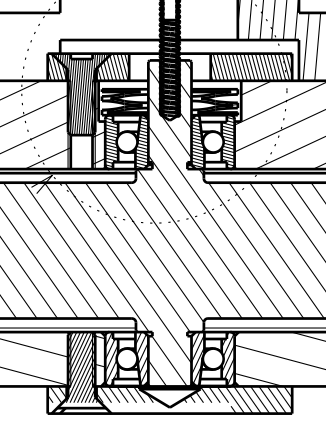
\includegraphics[width=0.7\linewidth]{img/dr27_cor}\end{center}}

\ifdef{\public}{\newpage}{}

\end{document}
